\documentclass[a4paper, 12pt]{article}
\usepackage[utf8x]{inputenc}
\usepackage[english, russian]{babel}
\usepackage[left=25mm, top=25mm, right=25mm, bottom=25mm]{geometry}
\usepackage{cmap}
\usepackage{indentfirst}
\usepackage{tikz}
\usepackage{float}
\usepackage{amsmath, amsfonts, amssymb}
\usepackage{graphicx}
\usepackage{hyperref}
\usepackage{listings}
\usepackage{caption}
\usepackage{subcaption}
\usepackage{xcolor}
\usepackage{etoolbox}
\usepackage{titlesec}
\usepackage{array}
\pagestyle{plain}
\patchcmd{\tableofcontents}{\contentsname}{\centering\contentsname}{}{}
\titleformat{\section}[block]{\normalfont\large\bfseries\centering}{}{0pt}{}
\titleformat{\subsection}[block]{\normalfont\normalsize\bfseries\centering}{}{0pt}{}
\allowdisplaybreaks
\graphicspath{{src/images/}}
\usetikzlibrary{patterns}
\definecolor{LightGray}{gray}{0.95}
\definecolor{LightGray2}{gray}{0.7}
\hypersetup{
    colorlinks=true,
    linkcolor=blue,
    filecolor=magenta,
    urlcolor=cyan,
    pdftitle={contents setup},
    pdfpagemode=FullScreen,
}


\begin{document}
    \begin{titlepage}

        \begin{center}
        Федеральное государственное автономное образовательное учреждение высшего образования
        «Национальный Исследовательский Университет ИТМО»
        \vfill
        
        
\includegraphics[width=0.3\textwidth]{itmo.png} % requires /src/images/itmo.png

        {\large\bf ЛАБОРАТОРНАЯ РАБОТА №2}\\
        {\large\bf ПРЕДМЕТ «ЭЛЕКТРОННЫЕ УСТРОЙСТВА СИСТЕМ УПРАВЛЕНИЯ»}\\
        {\large\bf ТЕМА «СТАБИЛИЗАТОРЫ НАПРЯЖЕНИЯ»}\\
        Вариант №5
        \vfill

        \begin{flushright}
            \begin{minipage}{.45\textwidth}
            {
                \hbox{Преподаватель:}
                \hbox{Жданов В. А.}
                \hbox{}
                \hbox{Выполнил:}
                \hbox{Румянцев А. А.}
                \hbox{}
                \hbox{Факультет: СУиР}
                \hbox{Группа: R3341}
                \hbox{Поток: ЭлУСУ R22 бак 1.2}
            }
            \end{minipage}
        \end{flushright}
        \vfill
  
        Санкт-Петербург\\
        2025
        \end{center}
    \end{titlepage}
    
    \tableofcontents

    \newpage
    \section{Цель работы}
    Цель работы -- исследование и сравнение характеристик различных схемных решений
    стабилизаторов на дискретных элементах и стабилизатора в интегральном исполнении.


    \section{Исходные данные}
    В таблице ниже представлены исходные данные для варианта №5
    \begin{center}
        \begin{tabular}{ | m{4em} | m{2em}| } 
        \hline
        $U_{\text{вых.}}$, В& $8$\\ 
        \hline
        $R_{\text{н.}}$, Ом& $3500$\\ 
        \hline
        $U_{\text{вх.}}$, В& $16$\\ 
        \hline
        \end{tabular}
    \end{center}


    \section{Исследование параметрического стабилизатора}
    \subsection{Выбор стабилитрона}
    Выходное напряжение (напряжение стабилизации) составляет 8 В, тогда возьмем стабилитрон типа EDZV8.2B $\Rightarrow U_{\text{ст.}}=8.2$ В.
    При подаче 8.2 В он начнет проводить ток (при $<8.2$ В ничего не будет делать, при $>8.2$ В <<сбросит>>
    лишнее напряжение через себя, удерживая на нагрузке примерно 8.2 В; теперь $U_{\text{вых.}}=8.2$ В). Этот стабилитрон имеет рассеиваемую
    мощность $P_\text{ст.}=0.15$ Вт, дифференциальное сопротивление $r_{\text{ст.}}=30$ Ом
    
    
    \subsection{Расчет параметров схемы}
    Рассчитаем максимальный ток, текущий
    через стабилитрон
    $$
    I_{\text{ст. макс.}}=\dfrac{P_{\text{ст.}}}{U_{\text{ст.}}}=\dfrac{0.15}{8.2}=0.0182926829\text{ А}
    $$
    Рассчитаем ток нагрузки
    $$
    I_{\text{н.}}=I_{\text{ст.}}=\dfrac{U_{\text{вых}}}{R_{\text{н.}}}=\dfrac{8.2}{3500}=0.0023428571\text{ А}
    $$
    Рассчитаем номинальное значение тока на стабилитроне
    $$
    I_{\text{ст. ном.}}=\dfrac{I_{\text{ст. макс.}}-I_{\text{ст.}}}{2}=\dfrac{0.018-0.002}{2}=0.0079749129\text{ А}
    $$
    Определим балластное сопротивление резистора
    $$
    R_{\text{б.}}=\dfrac{U_{\text{вх.}}-U_{\text{вых.}}}{I_{\text{ст. ном.}}+I_{\text{н.}}}=\dfrac{16-8.2}{0.008+0.002}=755.9773090503\text{ Ом}
    $$


    \subsection{Коэффициент стабилизации}
    Определим коэффициент стабилизации
    $$
    k_{\text{ст.}}=\left( 1-\dfrac{R_{\text{б.}}\left( I_\text{ст. ном.}+I_{\text{н.}} \right)}{U_{\text{вх.}}} \right)\cdot\dfrac{R_{\text{б.}}+r_{\text{ст.}}}{r_{\text{ст.}}},
    $$
    $$
    k_{\text{ст.}}=\left( 1-\dfrac{755.977\left( 0.008+0.002 \right)}{16} \right)\cdot\dfrac{755.977+30}{30}=13.4271123629;
    $$
    Посчитаем оценку $k_{\text{ст.}}$ (приближенно коэффициент стабилизации)
    $$
    \hat{k}_{\text{ст.}}=\dfrac{R_{\text{б.}}U_{\text{вых.}}}{r_{\text{ст.}}U_{\text{вх.}}}=12.9146123629
    $$


    \subsection{Коэффициент полезного действия}
    Определим коэффициент полезного действия
    $$
    \eta=\dfrac{I_\text{ст. ном.}U_{\text{ст.}}}{U_{\text{вх.}}\left( I_{\text{ст. ном.}}+I_{\text{н.}} \right)}=\dfrac{0.008\cdot8.2}{16\left( 0.008+0.002 \right)}=0.3961265720\approx40\%
    $$


    \subsection{Схема параметрического стабилизатора постоянного напряжения}
    Соберем схему параметрического стабилизатора постоянного напряжения с учетом наших расчетов.
    Конденсатор в расчетах не участвовал (со временем перестанет проводить ток)
    -- он нужен для сглаживания пульсаций (фильтр шумов)
    \begin{figure}[H]
        \centering
        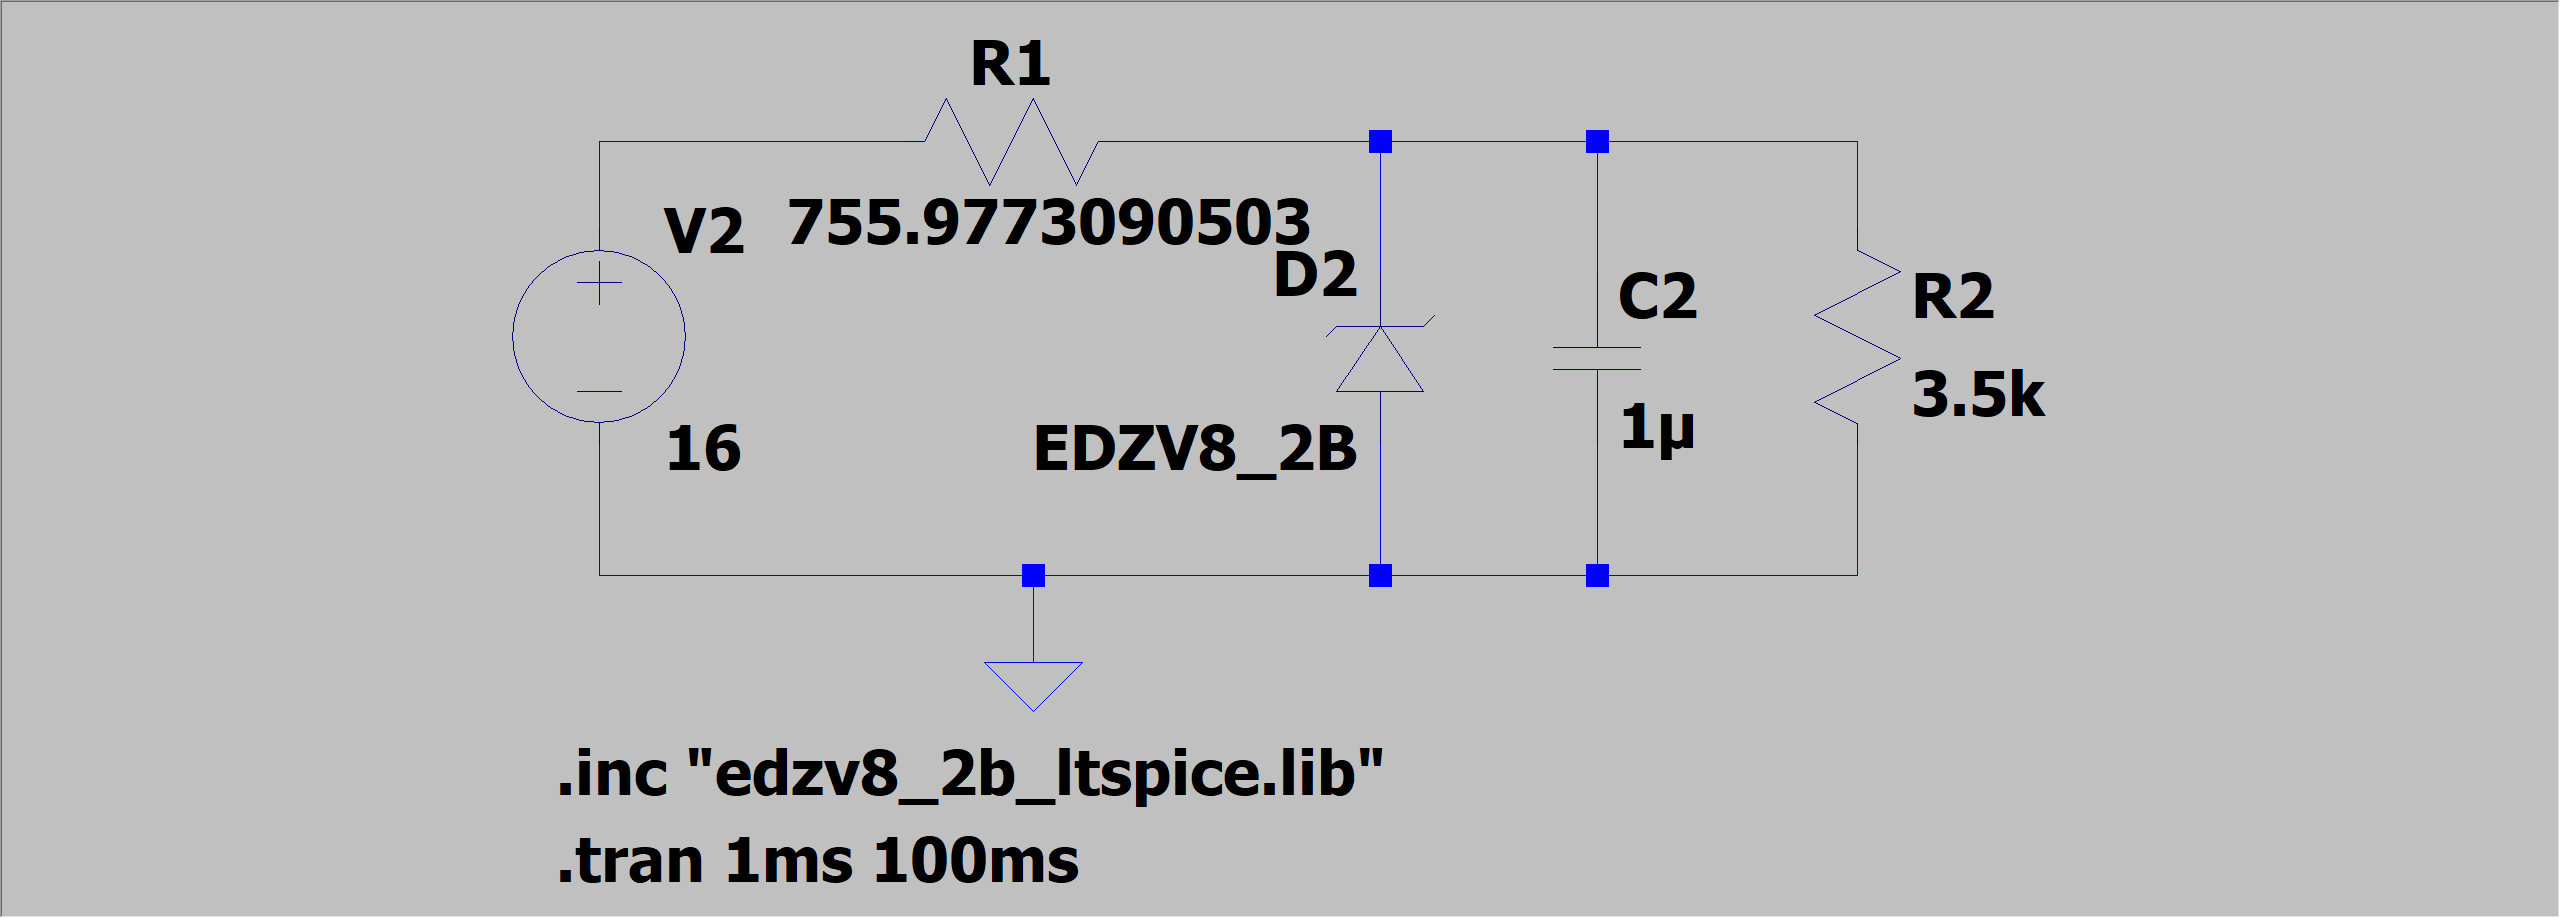
\includegraphics[scale=0.22]{1task_scheme_AC.png}
        \captionsetup{skip=0pt}
        \caption{Схема параметрического стабилизатора постоянного напряжения}
        \label{fig:1task_scheme_AC}
    \end{figure}


    \subsection{Влияние сопротивления нагрузки на работу стабилизатора}
    Проверим выходное напряжение цепи и ток на стабилизаторе при постоянном входном напряжении
    16 В и различных сопротивлениях нагрузки. V(n001)$\equiv U_{\text{вх.}}$, V(n002)$\equiv U_{\text{вых.}}$,
    I(D2)$\equiv I_{\text{ст.}}$. Результаты представлены на рис.
    \ref{fig:1task_R1k}--\ref{fig:1task_R100k}
    \begin{figure}[H]
        \centering
        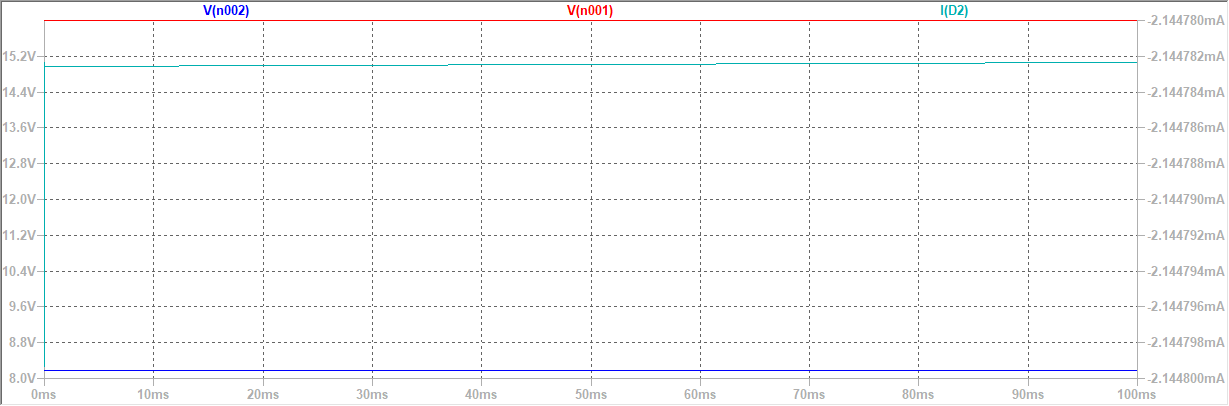
\includegraphics[scale=0.46]{1task_R1k.png}
        \captionsetup{skip=0pt}
        \caption{Выходное напряжение при $R_{\text{н.}}=1000$ Ом; $U_{\text{вых. ср.}}=8.1884$ В}
        \label{fig:1task_R1k}
    \end{figure}
    \begin{figure}[H]
        \centering
        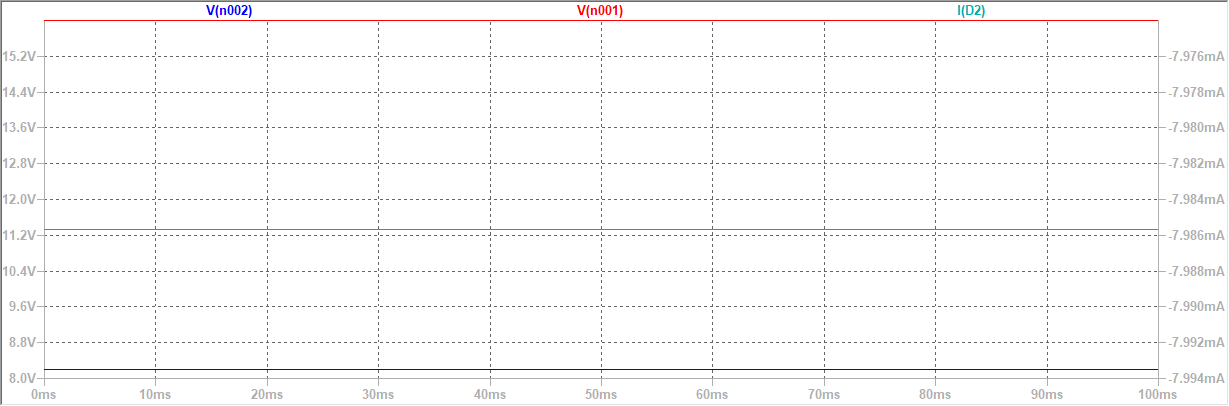
\includegraphics[scale=0.46]{1task_R3_5k.png}
        \captionsetup{skip=0pt}
        \caption{Выходное напряжение при $R_{\text{н.}}=3500$ Ом; $U_{\text{вых. ср.}}=8.1933$ В}
        \label{fig:1task_R3_5k}
    \end{figure}
    \begin{figure}[H]
        \centering
        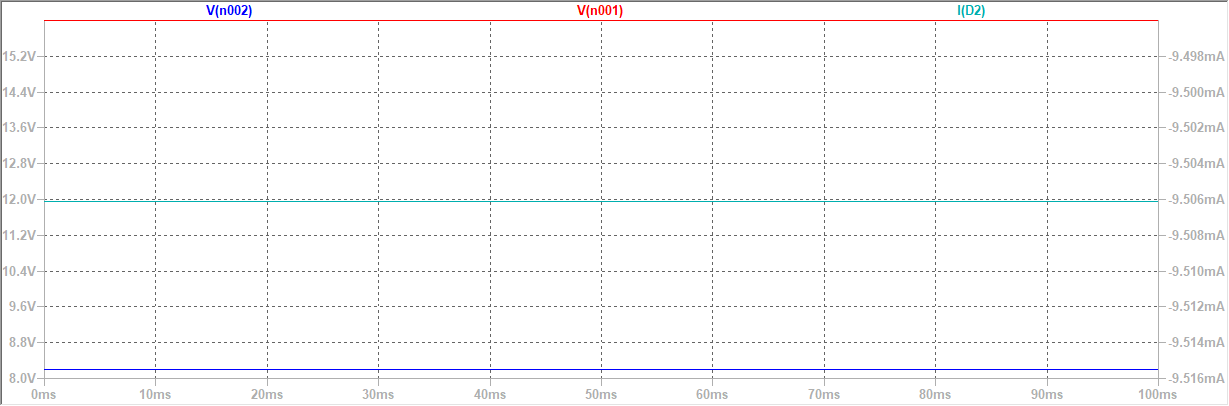
\includegraphics[scale=0.46]{1task_R10k.png}
        \captionsetup{skip=0pt}
        \caption{Выходное напряжение при $R_{\text{н.}}=10000$ Ом; $U_{\text{вых. ср.}}=8.1941$ В}
        \label{fig:1task_R10k}
    \end{figure}
    \begin{figure}[H]
        \centering
        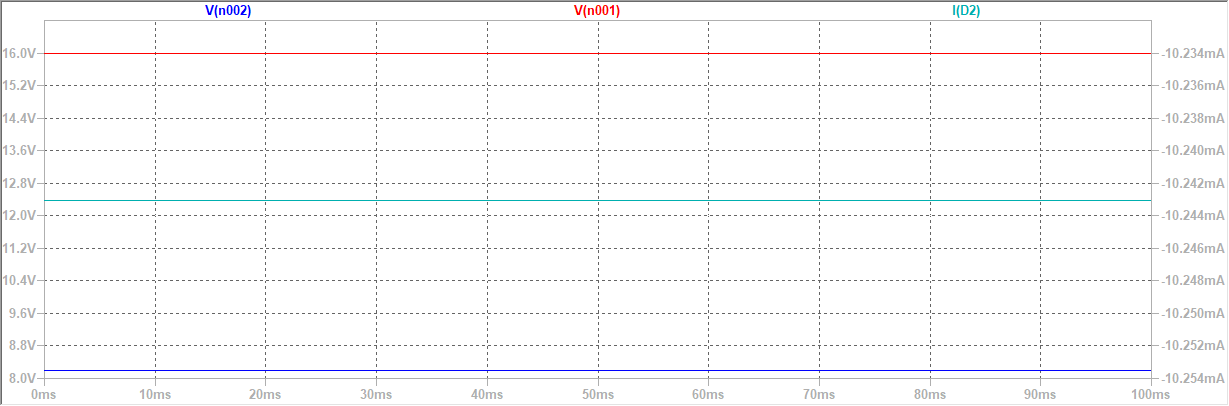
\includegraphics[scale=0.46]{1task_R100k.png}
        \captionsetup{skip=0pt}
        \caption{Выходное напряжение при $R_{\text{н.}}=100000$ Ом; $U_{\text{вых. ср.}}=8.1945$ В}
        \label{fig:1task_R100k}
    \end{figure}
    \noindent Выходное напряжение с увеличением сопротивления нагрузки немного увеличивается,
    при этом стабилитрон потребляет больше тока. Максимальное значение тока на стабилитроне в 18 мА
    не было достигнуто (при $R_{\text{н.}}=100000$ Ом получили $I_{\text{ст.}}\approx10.243$ мА).


    \subsection{Скачкообразное изменение нагрузки}
    Подадим скачкообразную нагрузку PULSE(16 18 5m 1u 1u 10m 10m). Входное напряжение
    представлено на рис. \ref{fig:1task_rect_input0}
    \begin{figure}[H]
        \centering
        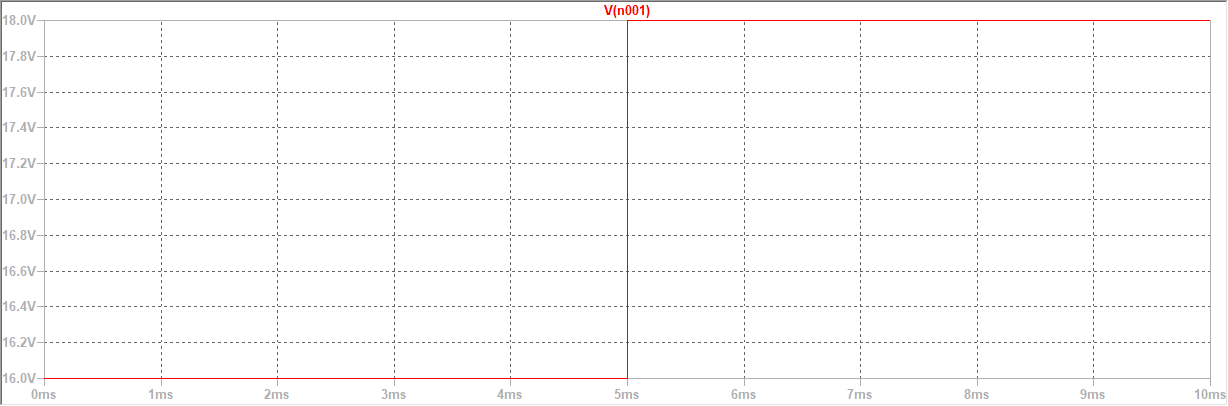
\includegraphics[scale=0.46]{1task_rect_input0.png}
        \captionsetup{skip=0pt}
        \caption{Скачкообразная нагрузка с 16 В до 18 В}
        \label{fig:1task_rect_input0}
    \end{figure}
    При таком входном напряжении на выходе получаем
    \begin{figure}[H]
        \centering
        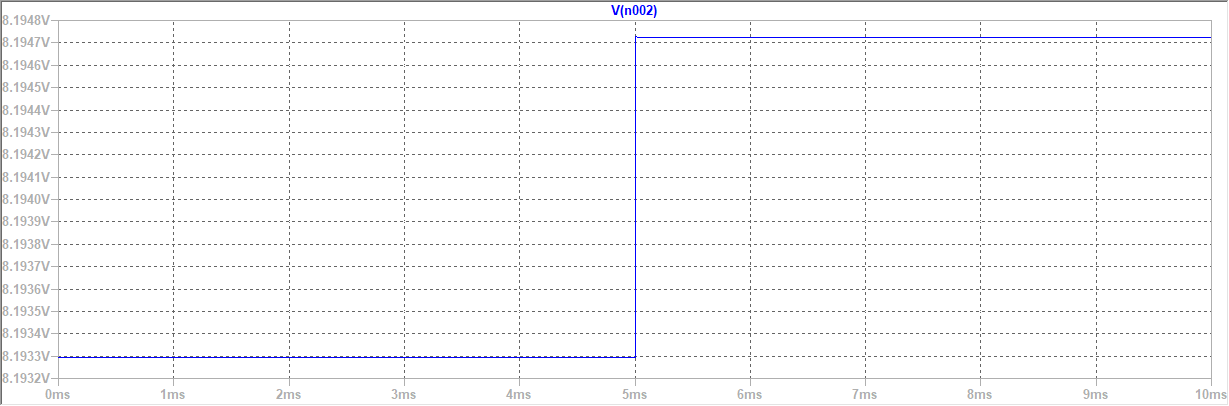
\includegraphics[scale=0.46]{1task_rect.png}
        \captionsetup{skip=0pt}
        \caption{Выходное напряжение при скачкообразной нагрузке}
        \label{fig:1task_rect}
    \end{figure}
    \noindent Скачок напряжения на выходе значительно меньше скачка на входе. Стабилизатор
    удержал напряжение в районе 8.2 В.


    \subsection{Нагрузки разного вида при скачкообразном изменении входного напряжения}
    Снимем осциллограммы выходных напряжений стабилизатора при скачкообразном
    изменении входного напряжения для нагрузок разного вида. На схеме на рис. \ref{fig:1task_scheme_AC}
    представлена активно-емкостная нагрузка. Для начала построим схему только лишь \textbf{активной} нагрузки
    \begin{figure}[H]
        \centering
        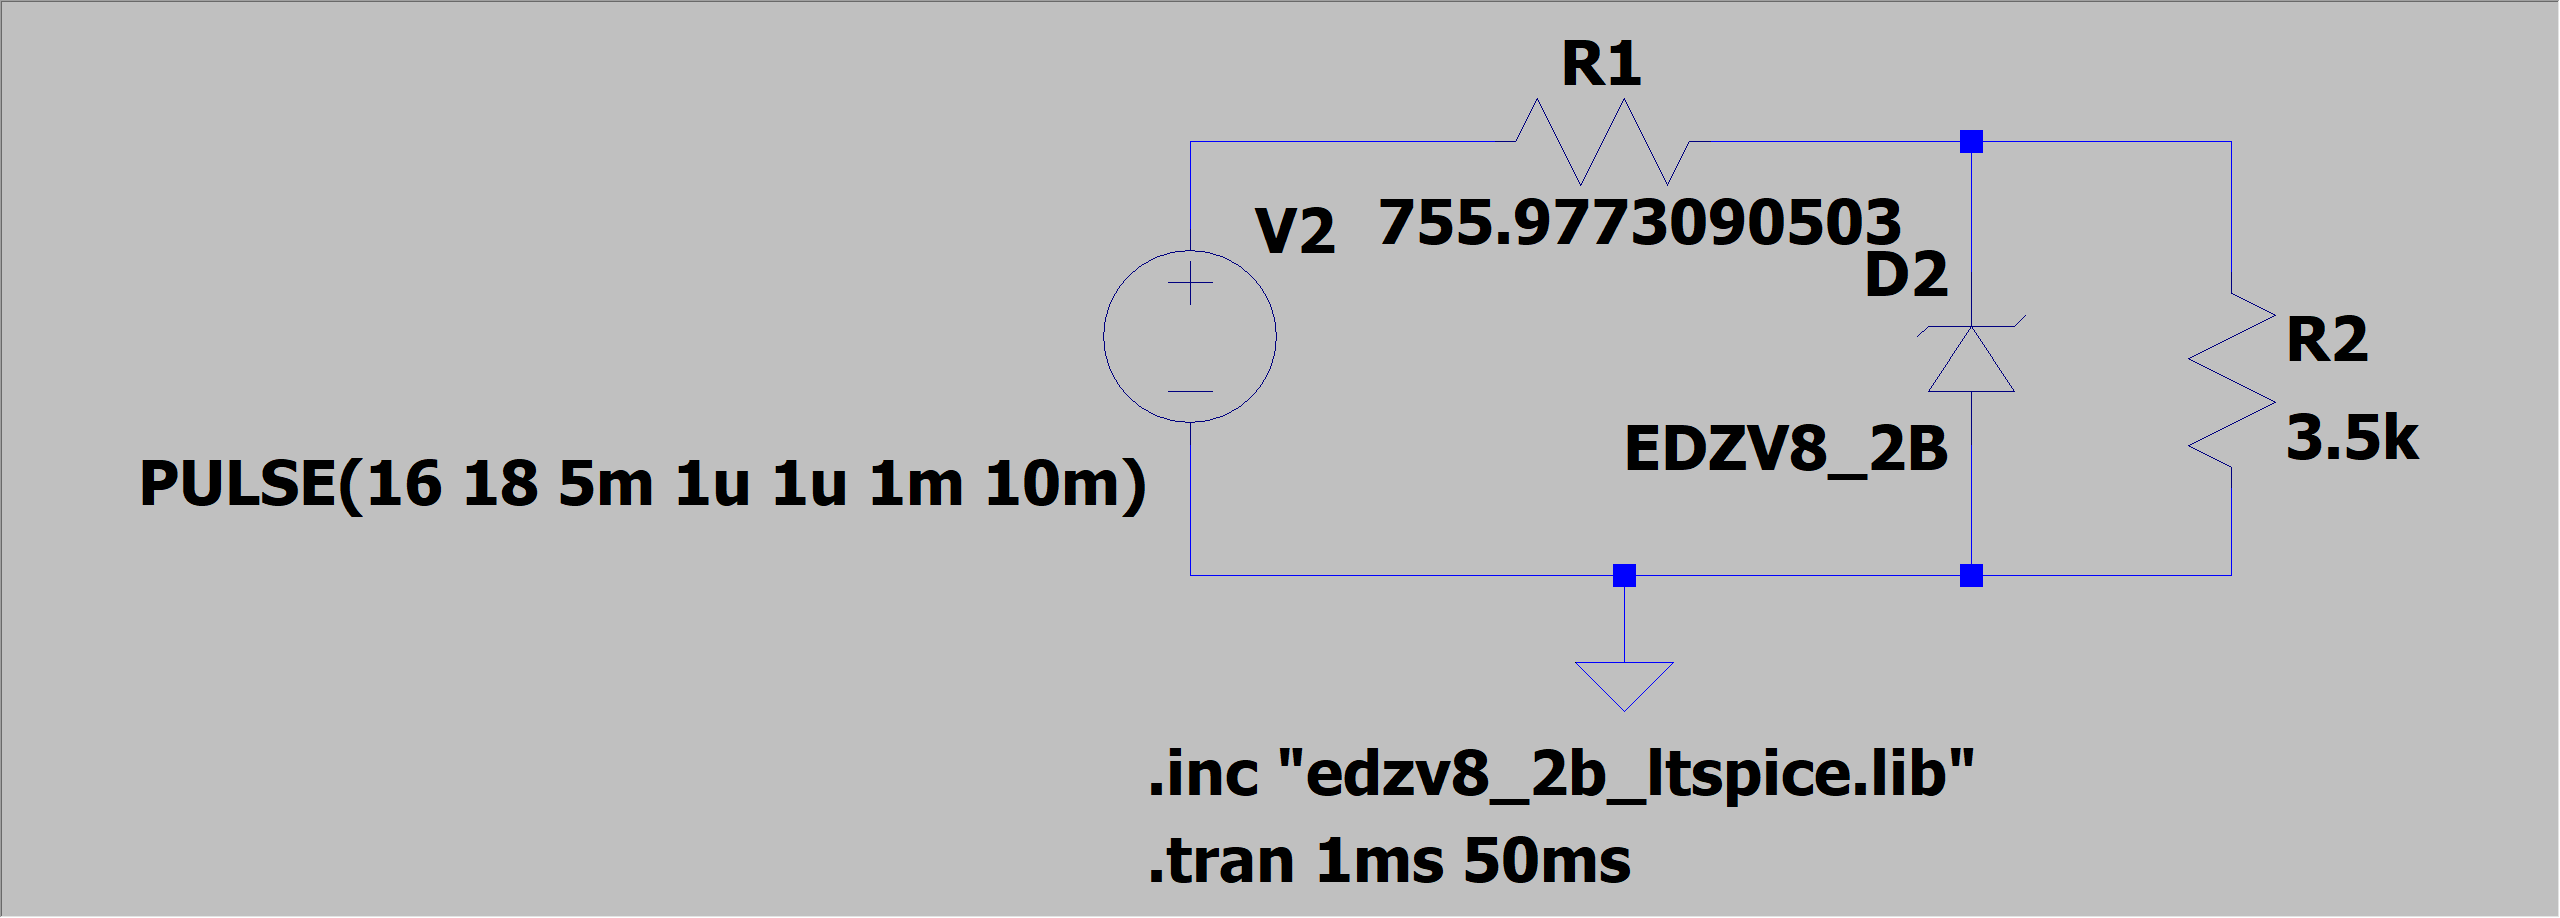
\includegraphics[scale=0.22]{1task_scheme_A.png}
        \captionsetup{skip=0pt}
        \caption{Схема параметрического стабилизатора: активная нагрузка}
        \label{fig:1task_scheme_A}
    \end{figure}
    \noindent Подадим на вход скачкообразный сигнал PULSE(16 18 5m 1u 1u 1m 10m), который
    представлен на рис. \ref{fig:1task_rect_input}
    \begin{figure}[H]
        \centering
        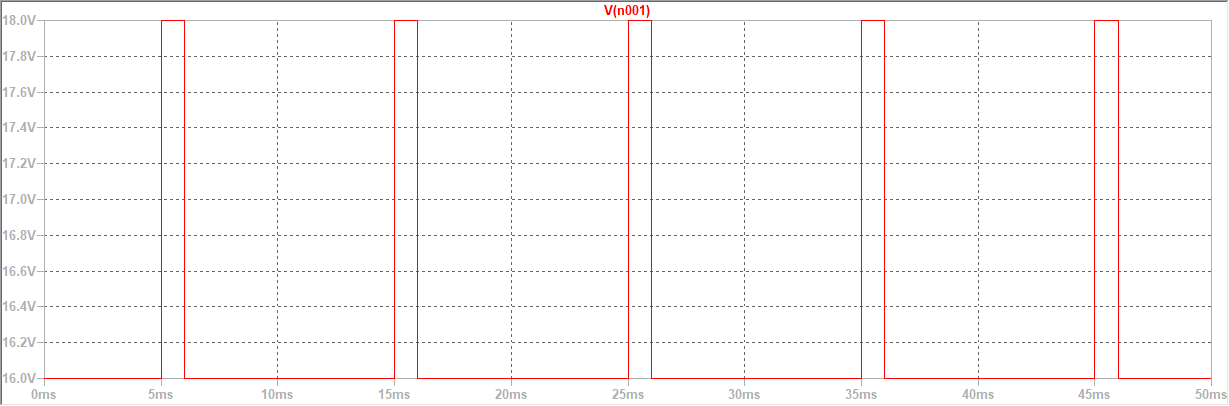
\includegraphics[scale=0.46]{1task_rect_input.png}
        \captionsetup{skip=0pt}
        \caption{Повторяющаяся скачкообразная нагрузка с 16 В до 18 В}
        \label{fig:1task_rect_input}
    \end{figure}
    Посмотрим выходное напряжение при \textbf{активной} скачкообразной нагрузке
    \begin{figure}[H]
        \centering
        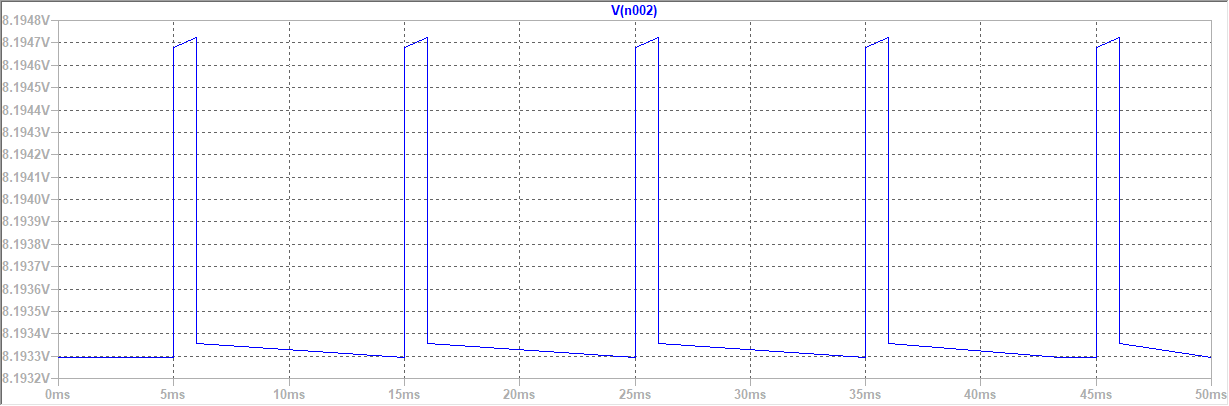
\includegraphics[scale=0.46]{1task_rect_A.png}
        \captionsetup{skip=0pt}
        \caption{Выходное напряжение при активной скачкообразной нагрузке}
        \label{fig:1task_rect_A}
    \end{figure}
    \noindent Посмотрим выходное напряжение при \textbf{активно-емкостной} нагрузке. Схема
    была представлена на рис. \ref{fig:1task_scheme_AC}
    \begin{figure}[H]
        \centering
        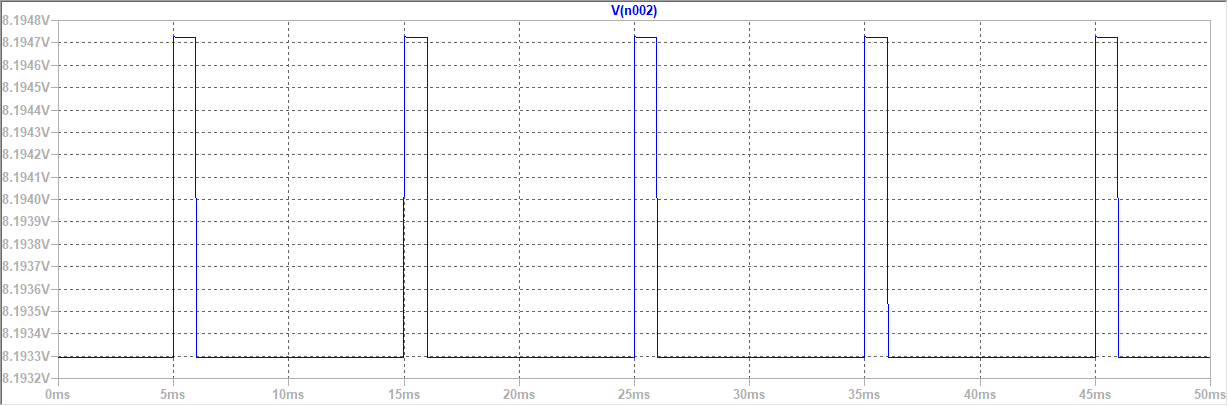
\includegraphics[scale=0.46]{1task_rect_AC.png}
        \captionsetup{skip=0pt}
        \caption{Выходное напряжение при активно-емкостной скачкообразной нагрузке}
        \label{fig:1task_rect_AC}
    \end{figure}
    \noindent Построим схему для проверки \textbf{активно-индуктивной} нагрузки. Зададим
    значение индуктивности в 1 Гн
    \begin{figure}[H]
        \centering
        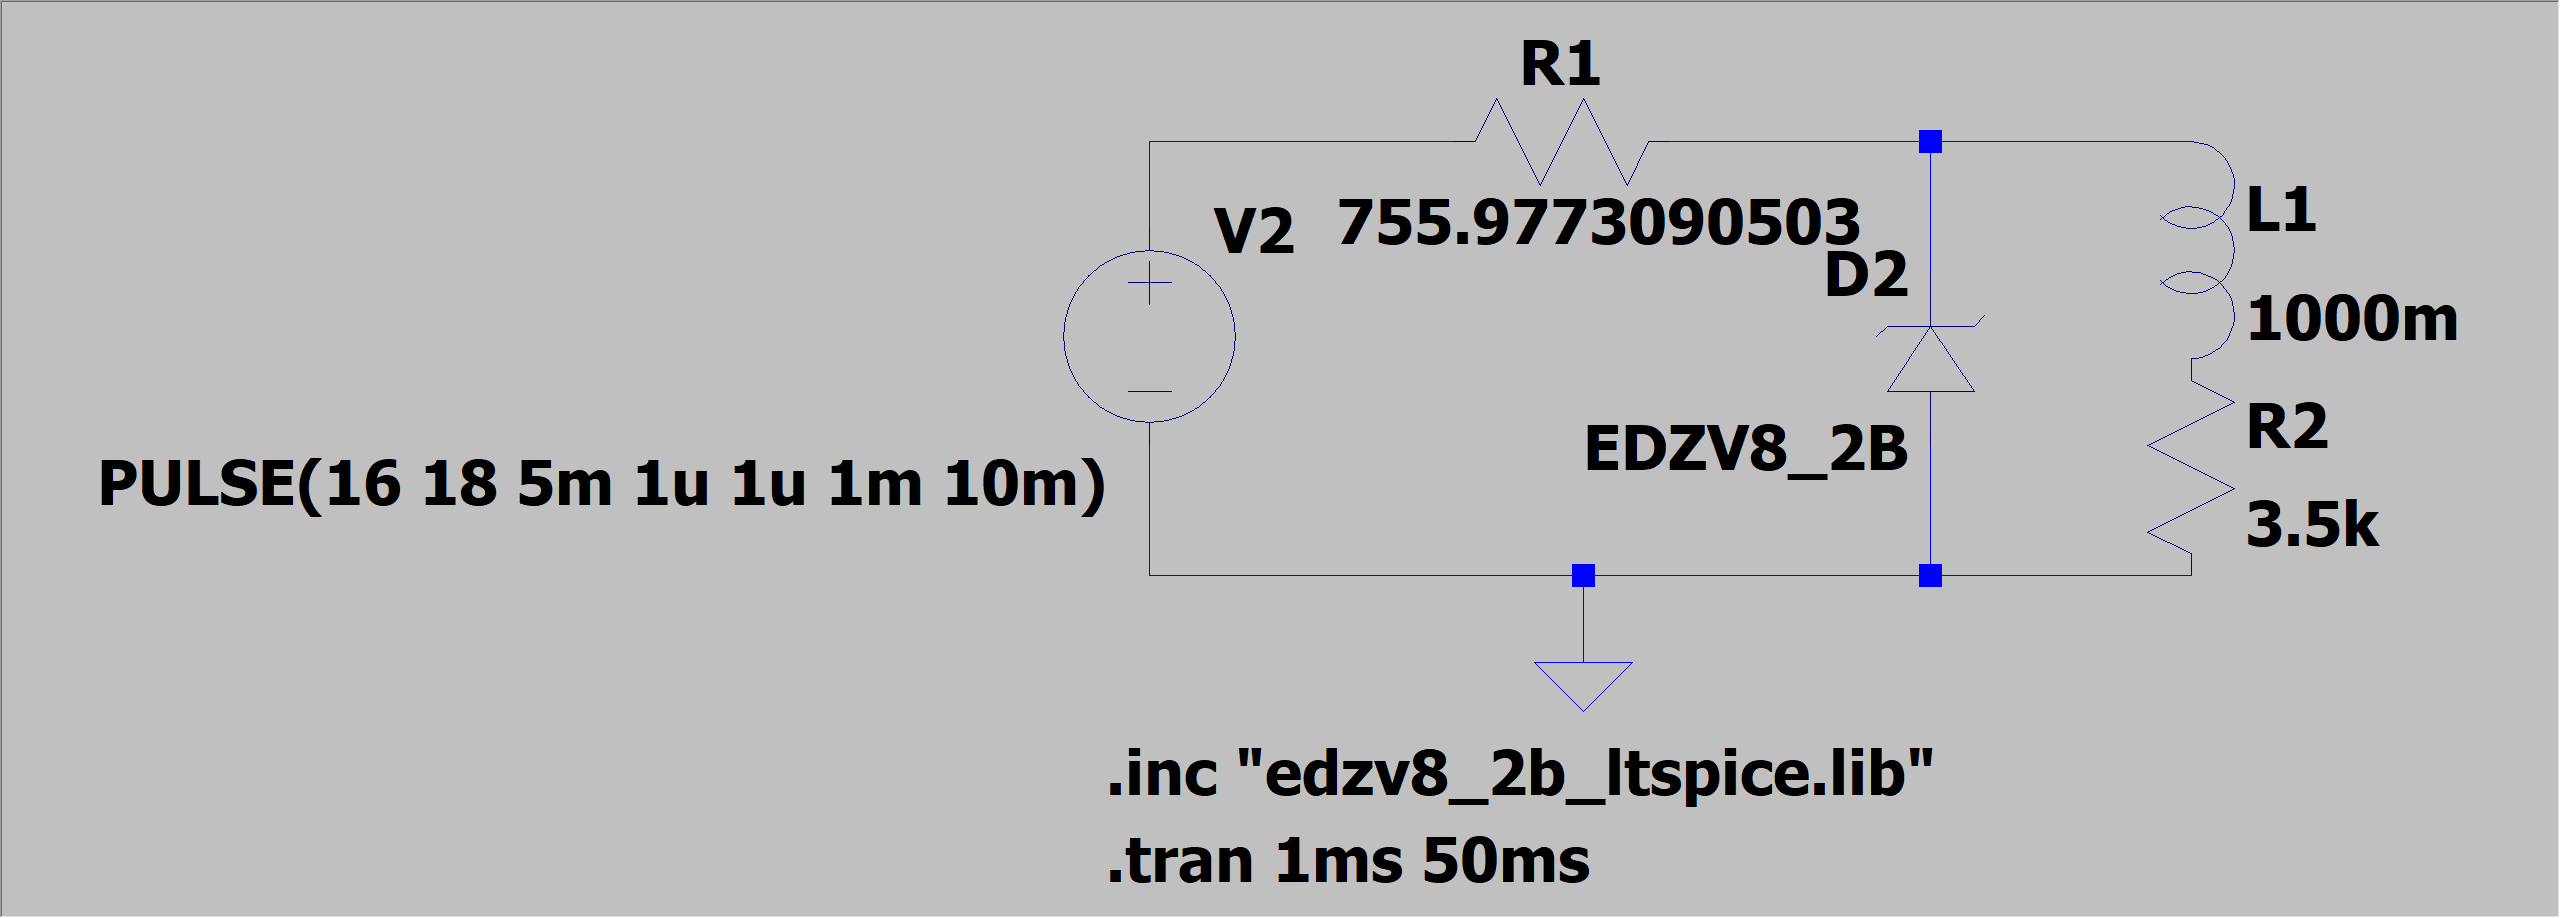
\includegraphics[scale=0.22]{1task_scheme_AL.png}
        \captionsetup{skip=0pt}
        \caption{Схема параметрического стабилизатора: активно-индуктивная нагрузка}
        \label{fig:1task_scheme_AL}
    \end{figure}
    \noindent Посмотрим выходное напряжение при \textbf{активно-индуктивной} нагрузке
    \begin{figure}[H]
        \centering
        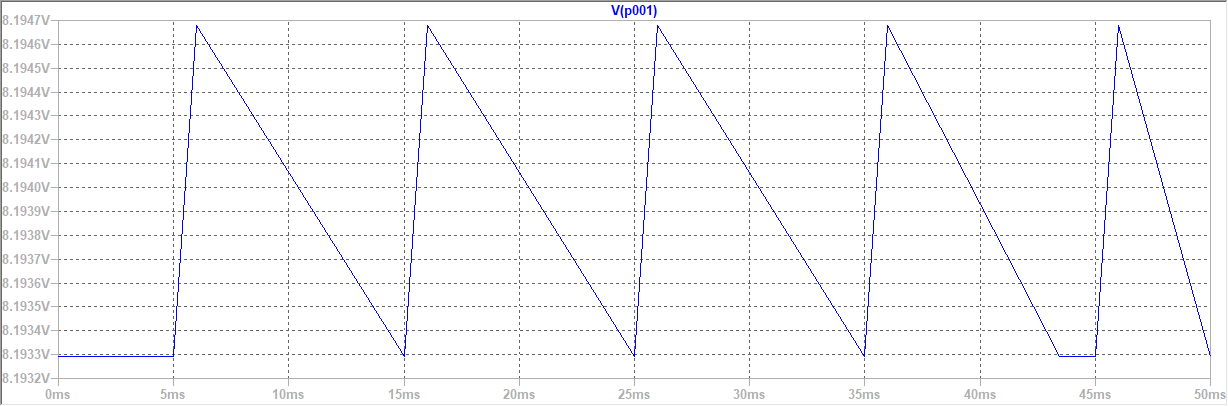
\includegraphics[scale=0.46]{1task_rect_AL.png}
        \captionsetup{skip=0pt}
        \caption{Выходное напряжение при активно-индуктивной скачкообразной нагрузке}
        \label{fig:1task_rect_AL}
    \end{figure}
    \noindent Построим схему для проверки \textbf{активно-индуктивно-емкостной} нагрузки. Зададим
    значение индуктивности в 1 Гн
    \begin{figure}[H]
        \centering
        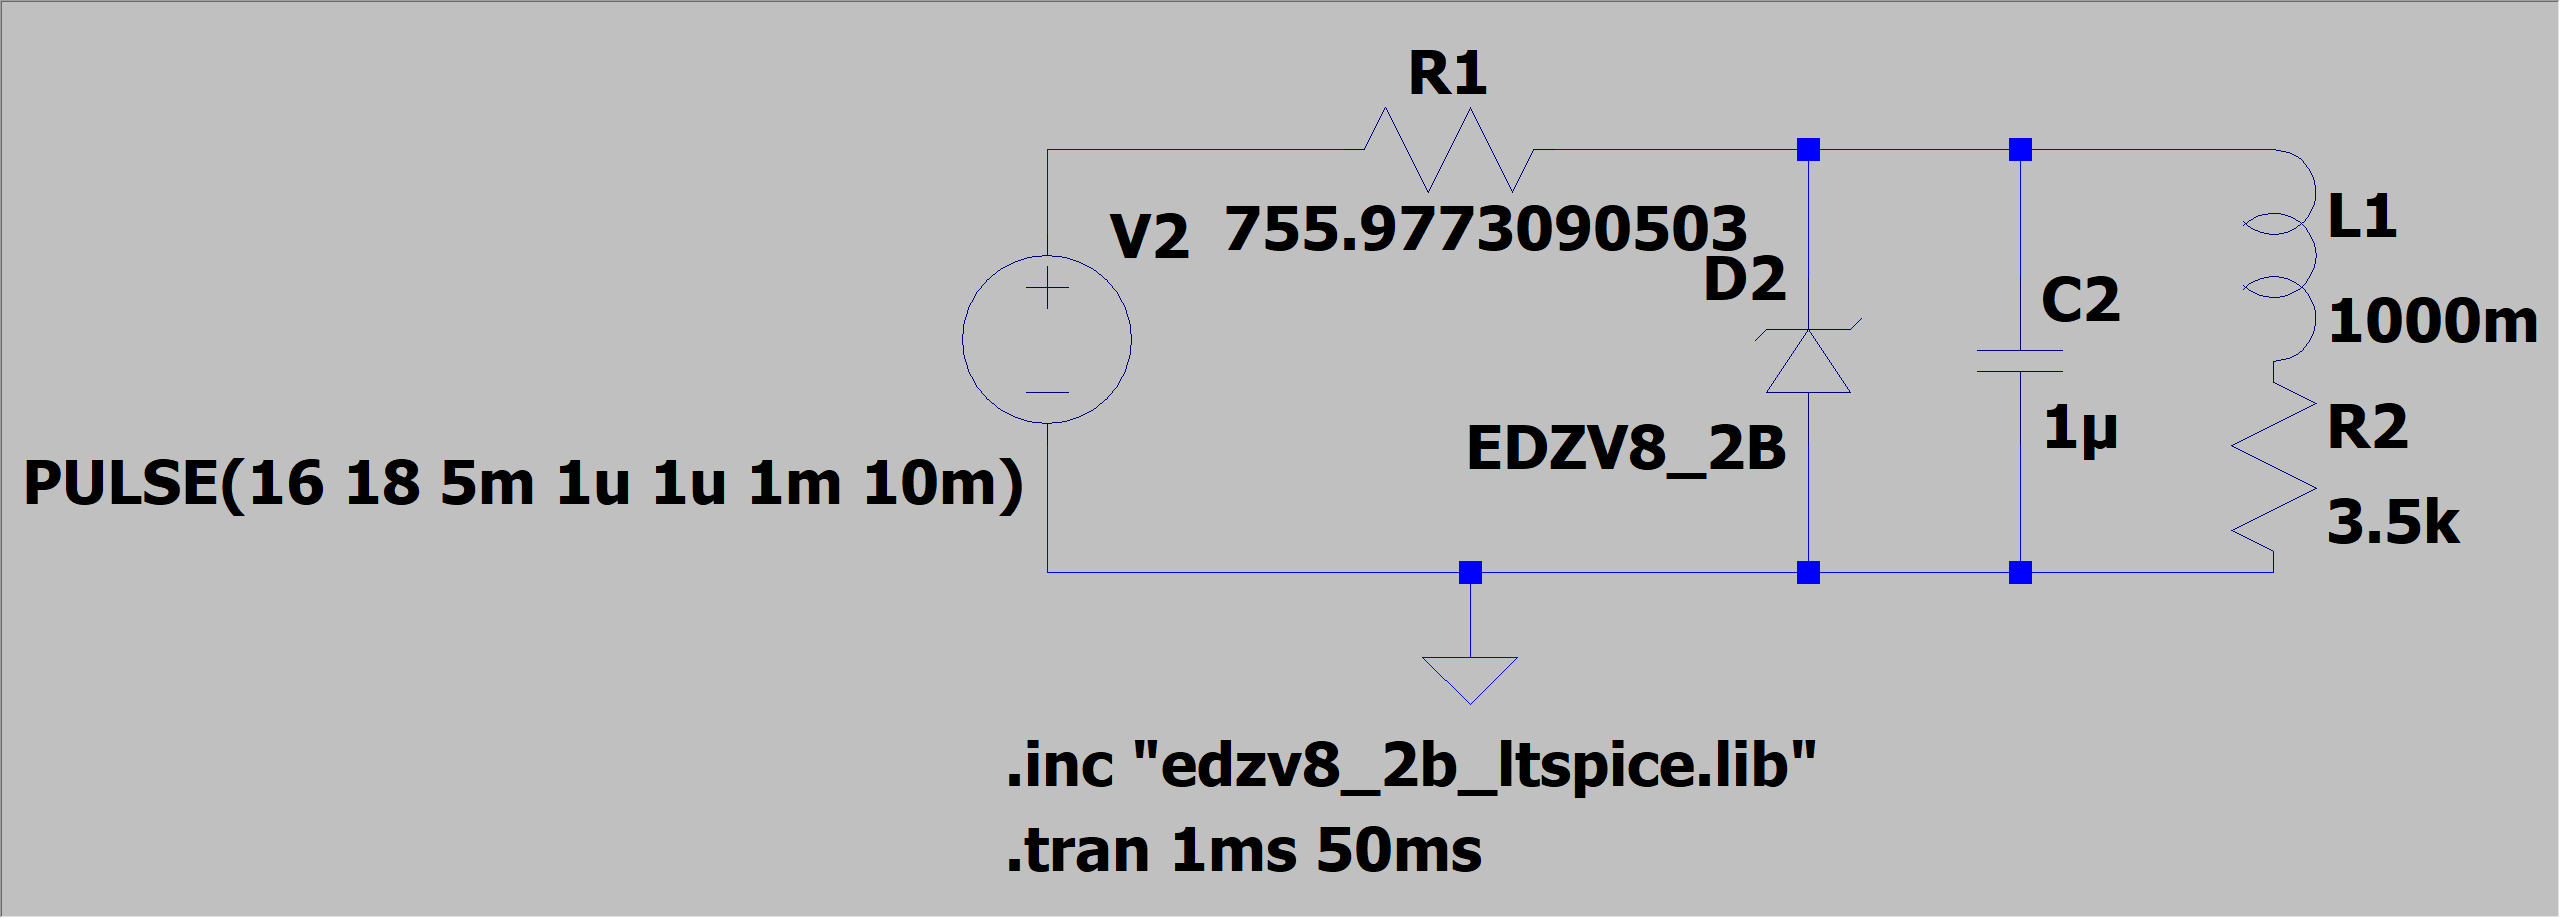
\includegraphics[scale=0.22]{1task_scheme_ALC.png}
        \captionsetup{skip=0pt}
        \caption{Схема параметрического стабилизатора: активно-индуктивно-емкостная нагрузка}
        \label{fig:1task_scheme_ALC}
    \end{figure}
    \noindent Посмотрим выходное напряжение при \textbf{активно-индуктивно-емкостной} нагрузке
    \begin{figure}[H]
        \centering
        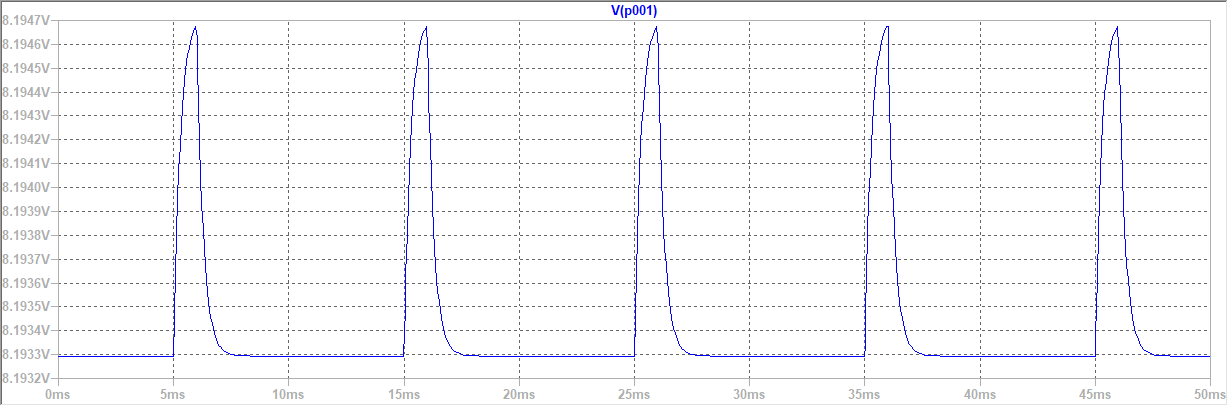
\includegraphics[scale=0.46]{1task_rect_ALC.png}
        \captionsetup{skip=0pt}
        \caption{Выходное напряжение при активно-индуктивно-емкостной скачкообразной нагрузке}
        \label{fig:1task_rect_ALC}
    \end{figure}
    \noindent Результат лучше всего получился на рис. \ref{fig:1task_rect_ALC}. При увеличении
    емкости конденсатора пульсации будут сглаживаться еще больше.


    \section{Исследование однотранзисторного последовательного линейного стабилизатора}
    \subsection{Выбор стабилитрона}
    Определимся со стабилизатором
    $$
    U_{\text{ст.}}=U_{\text{вых.}}+0.6=8+0.6=8.6\text{ В}
    $$
    Самые близкие доступные стабилизаторы -- EDZV8.2B на 8.2 В и EDZV9.1B на 9.1 В.
    Сравним по разнице между возможным и желаемым напряжениями на стабилизаторе и возьмем
    напряжение $U_{\text{ст.}}$, при котором разница наименьшая
    $$
    9.1-8.6=0.5,\ 8.2-8.6=-0.4,
    $$
    $$
    |-0.4|<|0.5|\Rightarrow\text{ берем EDZV8.2B}
    $$
    Пересчитаем выходное напряжение
    $$
    U_{\text{вых.}}=U_{\text{ст.}}-0.6=8.2-0.6=7.6\text{ В}
    $$
    В теории теряем 5\% от желаемых 8 В.
    
    
    \subsection{Расчет параметров схемы}
    Далее рассчитаем сопротивление на резисторе.
    Для транзистора 2N3055 выберем коэффициент передачи тока базы $h_{\text{FE мин.}}$
    $$\,20\leq h_{\text{FE}}\leq70\Rightarrow h_{\text{FE мин.}}=20$$
    Определим минимальное входное напряжение
    $$
    U_{\text{вх. мин.}}>U_{\text{вых.}}+2.5=7.6+2.5=10.1\Rightarrow U_{\text{вх. мин.}}=11\text{ В},
    $$
    Рассчитаем максимальный выходной ток стабилизатора
    $$
    I_{\text{вых. макс.}}=h_{\text{FE}}\cdot I_{\text{б.}},
    $$
    $$
    I_{\text{б. макс.}}\approx I_{\text{ст. макс.}}=\dfrac{P_{\text{ст.}}}{U_{\text{ст.}}}=\dfrac{0.15}{7.6}=0.0197368421\text{ А},
    $$
    $$
    I_{\text{вых. макс.}}=20\cdot0.02=0.394736842\text{ А}
    $$
    Теперь посчитаем $R$
    $$
    R\approx\dfrac{U_{\text{вх. мин.}}h_{\text{FE мин.}}}{1.2I_{\text{вых. макс.}}}=\dfrac{11\cdot20}{1.2\cdot0.395}=464.4444445683\text{ Ом}
    $$


    \subsection{Коэффициент стабилизации}
    Определим коэффициент стабилизации по формуле
    $$
    k_{\text{ст.}}=\dfrac{\Delta U_{\text{вх.}}}{U_{\text{вх.}}}\div\dfrac{\Delta U_{\text{вых.}}}{U_{\text{вых.}}}\bigg|_{\text{Rн=const.}}
    $$
    Значения $\Delta U_{\text{вых.}}$ возьмем с моделирования схемы, представленной на рис. \ref{fig:2task_scheme_AC}, в LTspice
    при $U_{\text{вх. 1}}=16$ В, $U_{\text{вх. 2}}=17$ В
    $$
    k_{\text{ст.}}=\dfrac{17-16}{16}\div\dfrac{7.9021-7.9013}{7.6}=593.7499999994
    $$


    \subsection{Схема однотранзисторного последовательного линейного стабилизатора постоянного напряжения}
    Построим схему однотранзисторного последовательного линейного стабилизатора постоянного напряжения, учитывая проведенные ранее расчеты
    \begin{figure}[H]
        \centering
        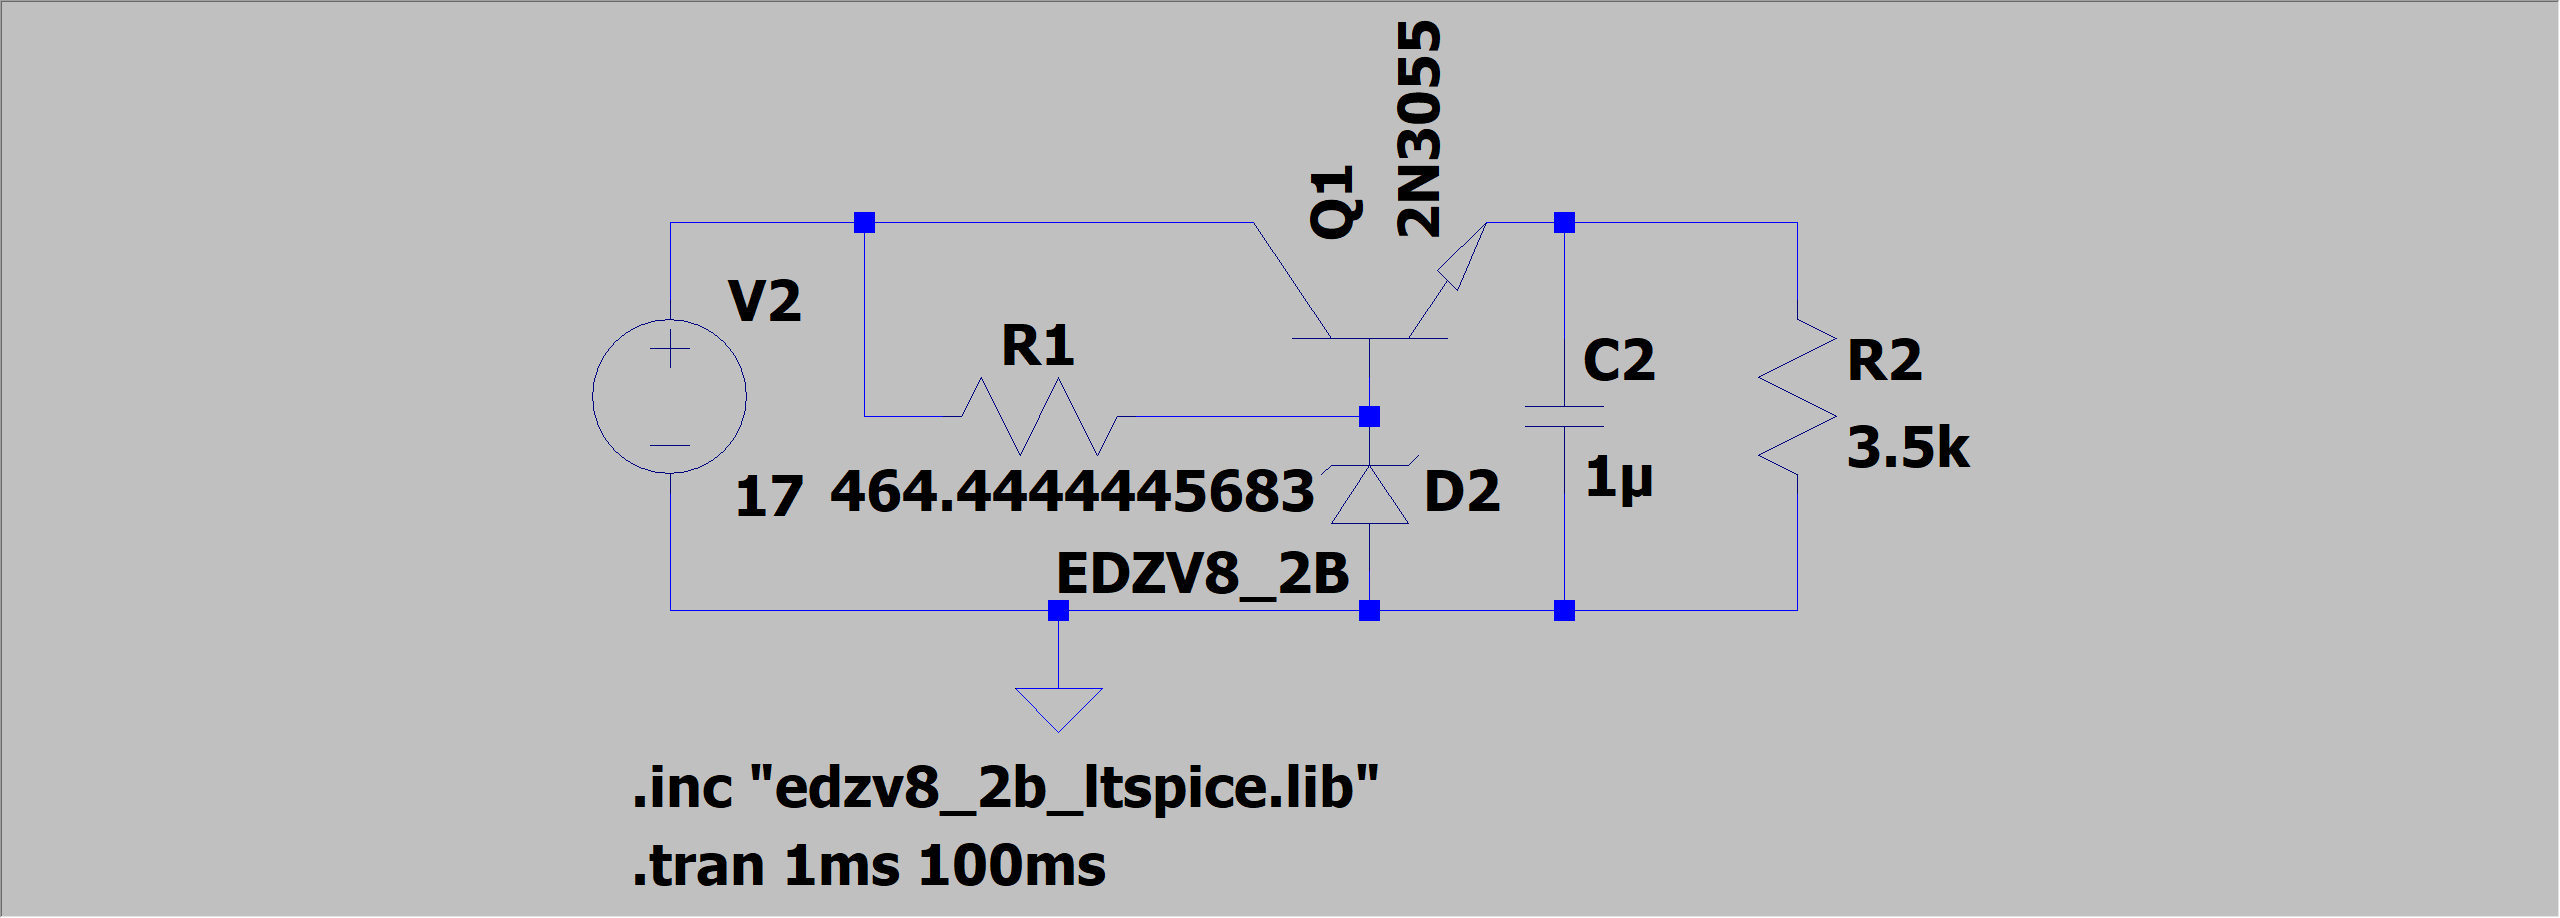
\includegraphics[scale=0.22]{2task_scheme_AC.png}
        \captionsetup{skip=0pt}
        \caption{Схема однотранзисторного последовательного линейного стабилизатора постоянного напряжения}
        \label{fig:2task_scheme_AC}
    \end{figure}


    \subsection{Влияние сопротивления нагрузки на работу стабилизатора}
    Проверим выходное напряжение цепи и ток на стабилизаторе при постоянном
    входном напряжении 16 В и различных сопротивлениях нагрузки. V(n001)$\equiv U_{\text{вх.}}$,
    V(n002)$\equiv U_{\text{вых.}}$, I(D2)$\equiv I_{\text{ст.}}$. Результаты представлены на рис.
    \ref{fig:2task_R1k}--\ref{fig:2task_R100k}
    \begin{figure}[H]
        \centering
        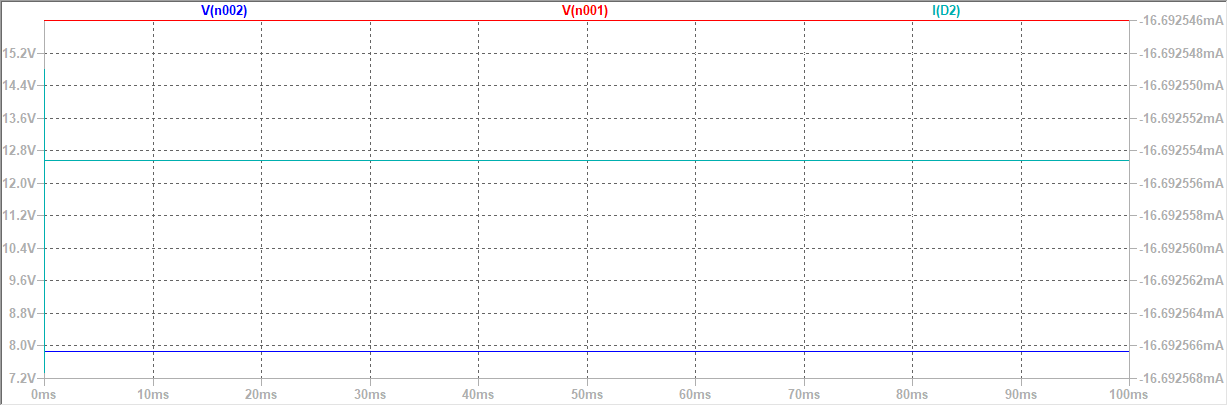
\includegraphics[scale=0.46]{2task_R1k.png}
        \captionsetup{skip=0pt}
        \caption{Выходное напряжение при $R_{\text{н.}}=1000$ Ом; $U_{\text{вых. ср.}}=7.8687$ В}
        \label{fig:2task_R1k}
    \end{figure}
    \begin{figure}[H]
        \centering
        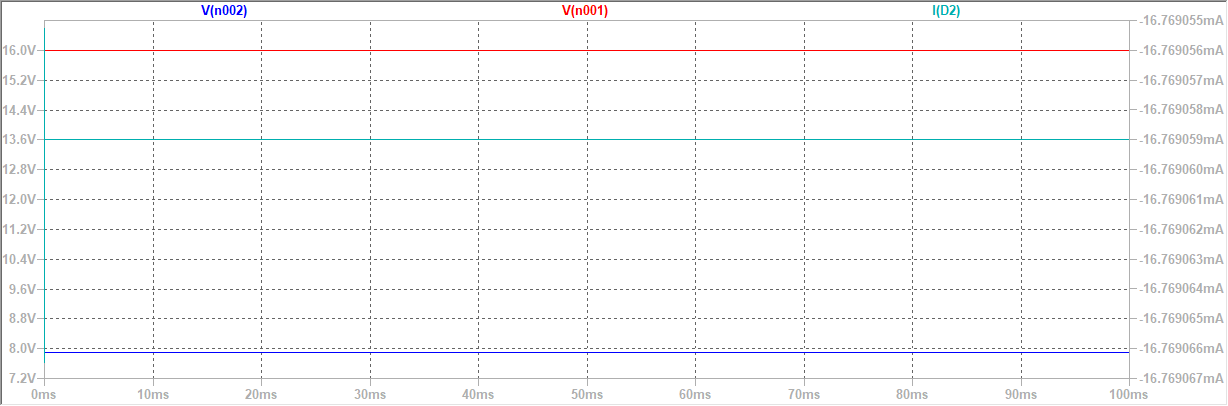
\includegraphics[scale=0.46]{2task_R3_5k.png}
        \captionsetup{skip=0pt}
        \caption{Выходное напряжение при $R_{\text{н.}}=3500$ Ом; $U_{\text{вых. ср.}}=7.9013$ В}
        \label{fig:2task_R3_5k}
    \end{figure}
    \begin{figure}[H]
        \centering
        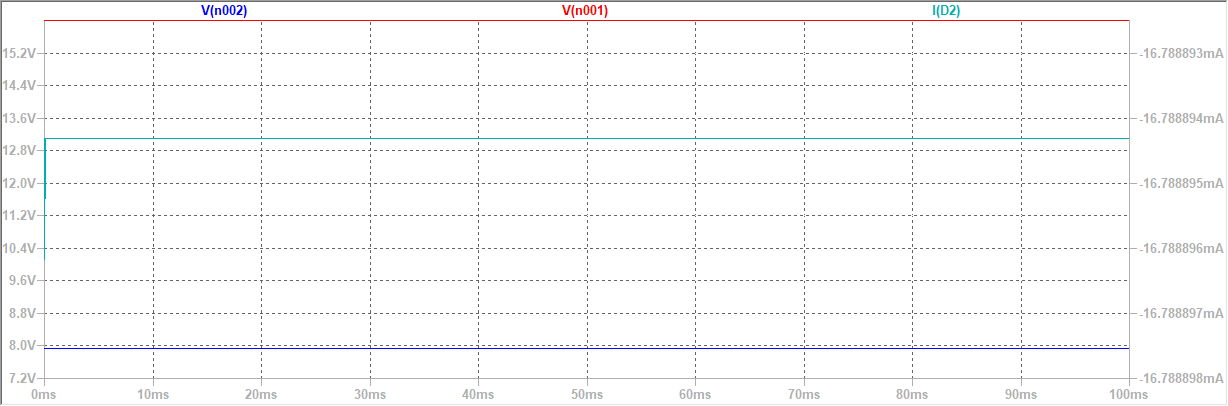
\includegraphics[scale=0.46]{2task_R10k.png}
        \captionsetup{skip=0pt}
        \caption{Выходное напряжение при $R_{\text{н.}}=10000$ Ом; $U_{\text{вых. ср.}}=7.9284$ В}
        \label{fig:2task_R10k}
    \end{figure}
    \begin{figure}[H]
        \centering
        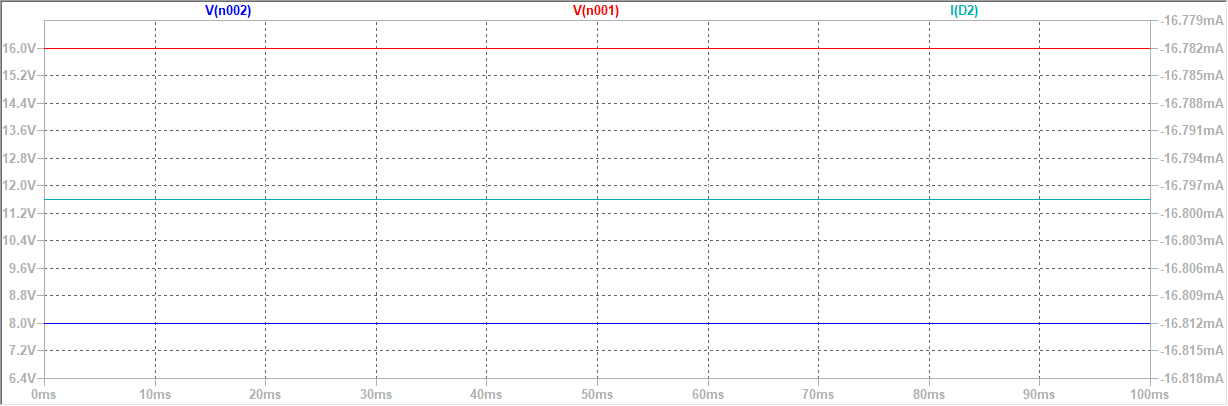
\includegraphics[scale=0.46]{2task_R100k.png}
        \captionsetup{skip=0pt}
        \caption{Выходное напряжение при $R_{\text{н.}}=100000$ Ом; $U_{\text{вых. ср.}}=7.9878$ В}
        \label{fig:2task_R100k}
    \end{figure}
    \noindent Выходное напряжение с увеличением сопротивления нагрузки немного увеличивается,
    при этом стабилитрон потребляет немного больше тока (в сравнении с результатами для первого задания, представленными
    на рис. \ref{fig:1task_R1k}--\ref{fig:1task_R100k}, увеличение потребления тока значительно меньше).


    \subsection{Скачкообразное изменение нагрузки}
    Выполним моделирование скачкообразного изменения нагрузки аналогично первому заданию
    (входное напряжение представлено на рис. \ref{fig:1task_rect_input0})
    \begin{figure}[H]
        \centering
        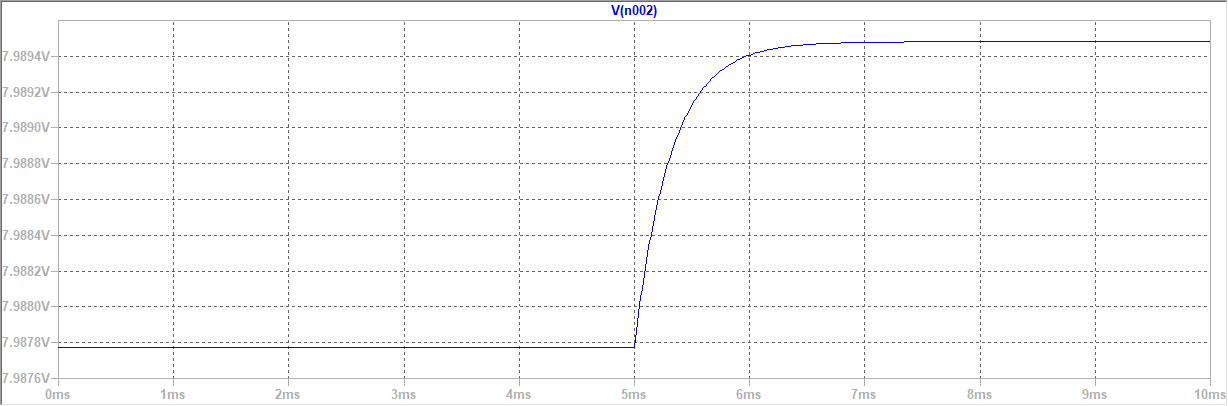
\includegraphics[scale=0.46]{2task_rect.png}
        \captionsetup{skip=0pt}
        \caption{Выходное напряжение при скачкообразной нагрузке}
        \label{fig:2task_rect}
    \end{figure}
    \noindent Скачок напряжения на выходе значительно меньше скачка на входе. Стабилизатор
    удержал напряжение в районе 8 В.


    \subsection{Нагрузки разного вида при скачкообразном изменении входного напряжения}
    Снимем осциллограммы выходных напряжений стабилизатора при скачкообразном
    изменении входного напряжения для нагрузок разного вида. На схеме на рис. \ref{fig:2task_scheme_AC}
    представлена активно-емкостная нагрузка. Для начала построим схему только лишь \textbf{активной} нагрузки
    \begin{figure}[H]
        \centering
        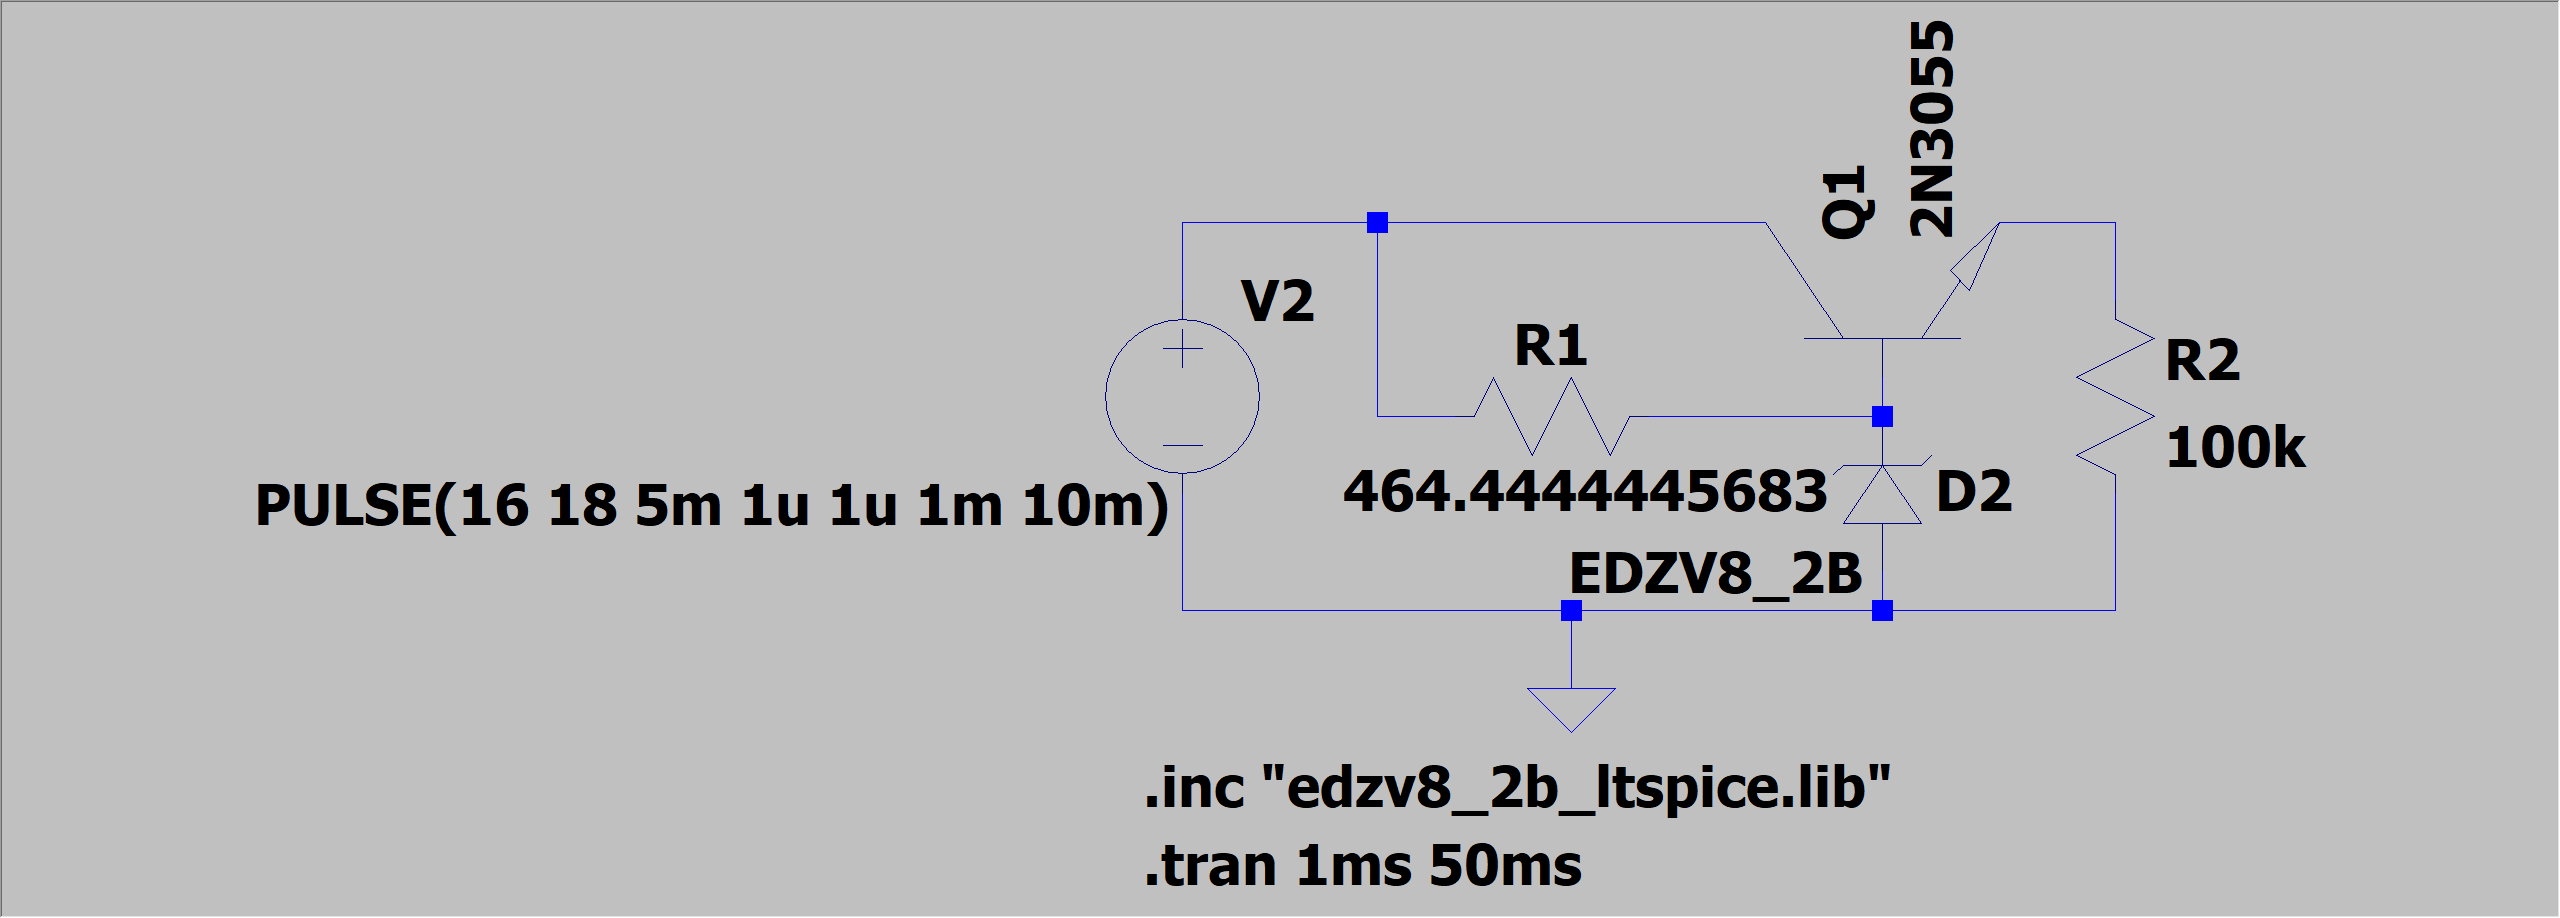
\includegraphics[scale=0.22]{2task_scheme_A.png}
        \captionsetup{skip=0pt}
        \caption{Схема параметрического стабилизатора: активная нагрузка}
        \label{fig:2task_scheme_A}
    \end{figure}
    \noindent Подадим на вход скачкообразный сигнал аналогично первому заданию (см рис. \ref{fig:1task_rect_input}).
    Посмотрим выходное напряжение при \textbf{активной} скачкообразной нагрузке
    \begin{figure}[H]
        \centering
        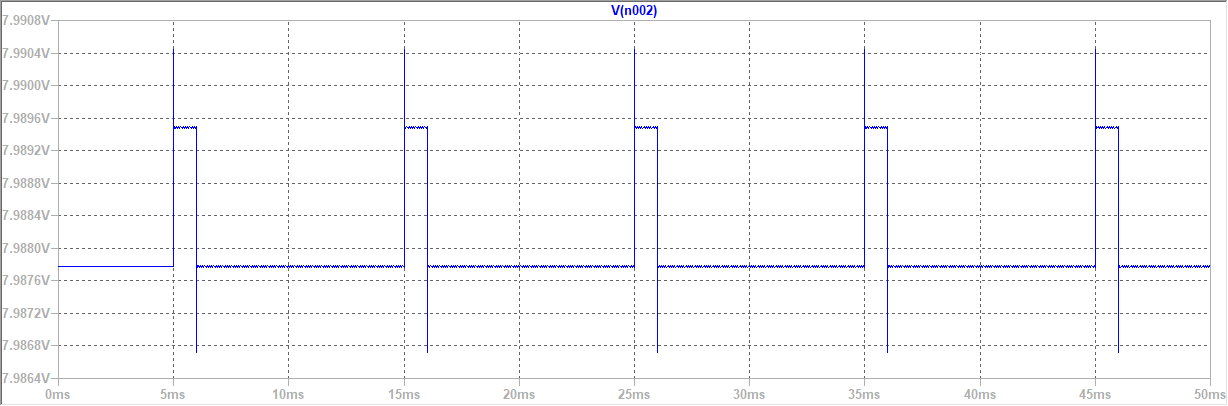
\includegraphics[scale=0.46]{2task_rect_A.png}
        \captionsetup{skip=0pt}
        \caption{Выходное напряжение при активной скачкообразной нагрузке}
        \label{fig:2task_rect_A}
    \end{figure}
    \noindent Посмотрим выходное напряжение при \textbf{активно-емкостной} нагрузке. Схема
    была представлена на рис. \ref{fig:2task_scheme_AC}
    \begin{figure}[H]
        \centering
        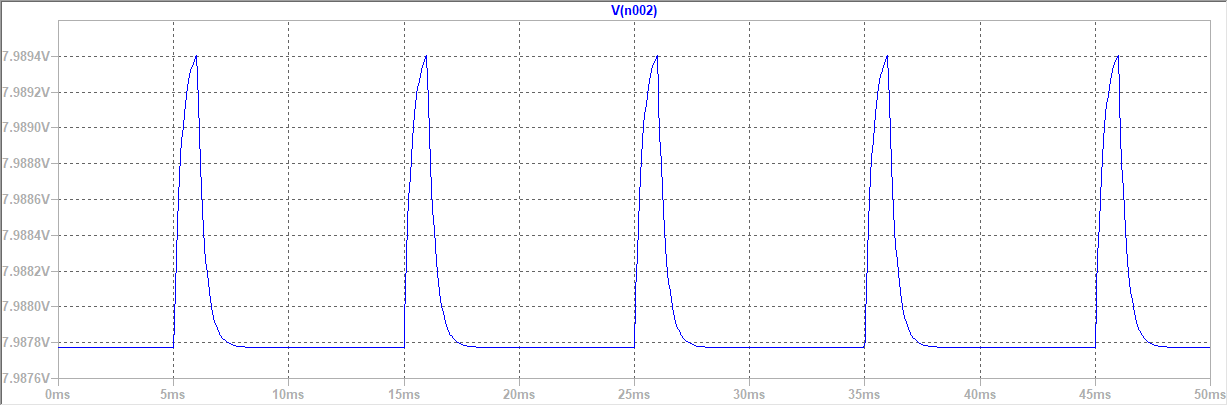
\includegraphics[scale=0.46]{2task_rect_AC.png}
        \captionsetup{skip=0pt}
        \caption{Выходное напряжение при активно-емкостной скачкообразной нагрузке}
        \label{fig:2task_rect_AC}
    \end{figure}
    \noindent Построим схему для проверки \textbf{активно-индуктивной} нагрузки. Зададим
    значение индуктивности в 100 Гн
    \begin{figure}[H]
        \centering
        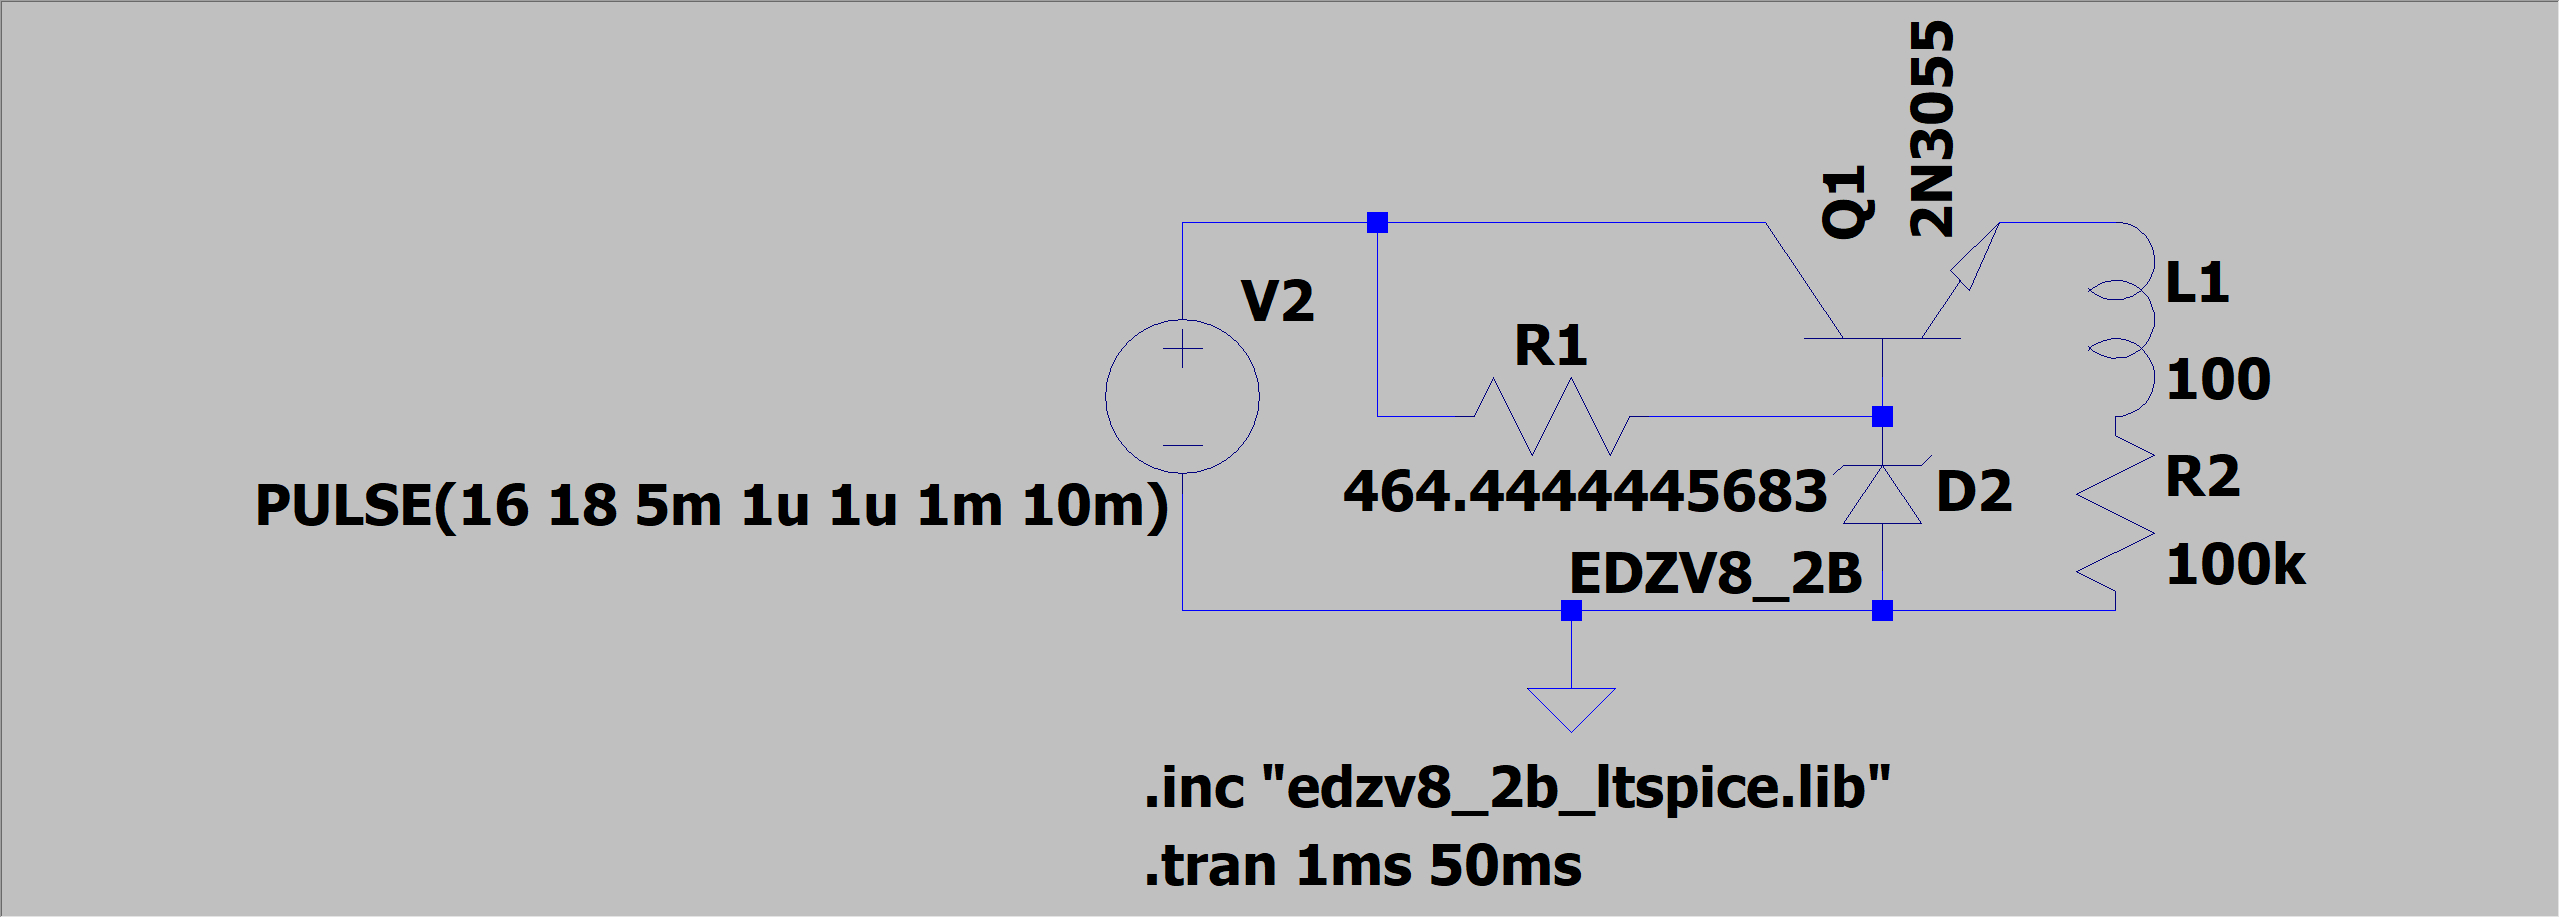
\includegraphics[scale=0.22]{2task_scheme_AL.png}
        \captionsetup{skip=0pt}
        \caption{Схема параметрического стабилизатора: активно-индуктивная нагрузка}
        \label{fig:2task_scheme_AL}
    \end{figure}
    \noindent Посмотрим выходное напряжение при \textbf{активно-индуктивной} нагрузке
    \begin{figure}[H]
        \centering
        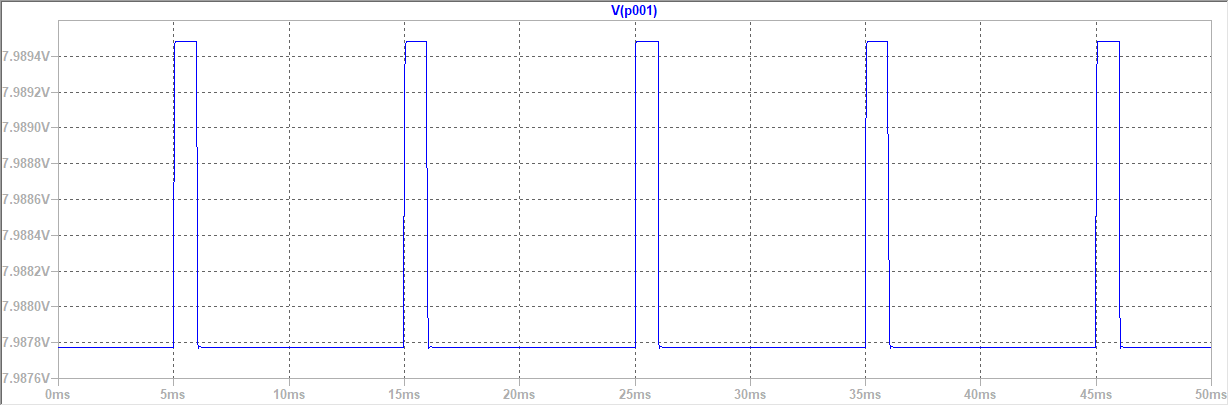
\includegraphics[scale=0.46]{2task_rect_AL.png}
        \captionsetup{skip=0pt}
        \caption{Выходное напряжение при активно-индуктивной скачкообразной нагрузке}
        \label{fig:2task_rect_AL}
    \end{figure}
    \noindent Построим схему для проверки \textbf{активно-индуктивно-емкостной} нагрузки. Зададим
    значение индуктивности в 100 Гн
    \begin{figure}[H]
        \centering
        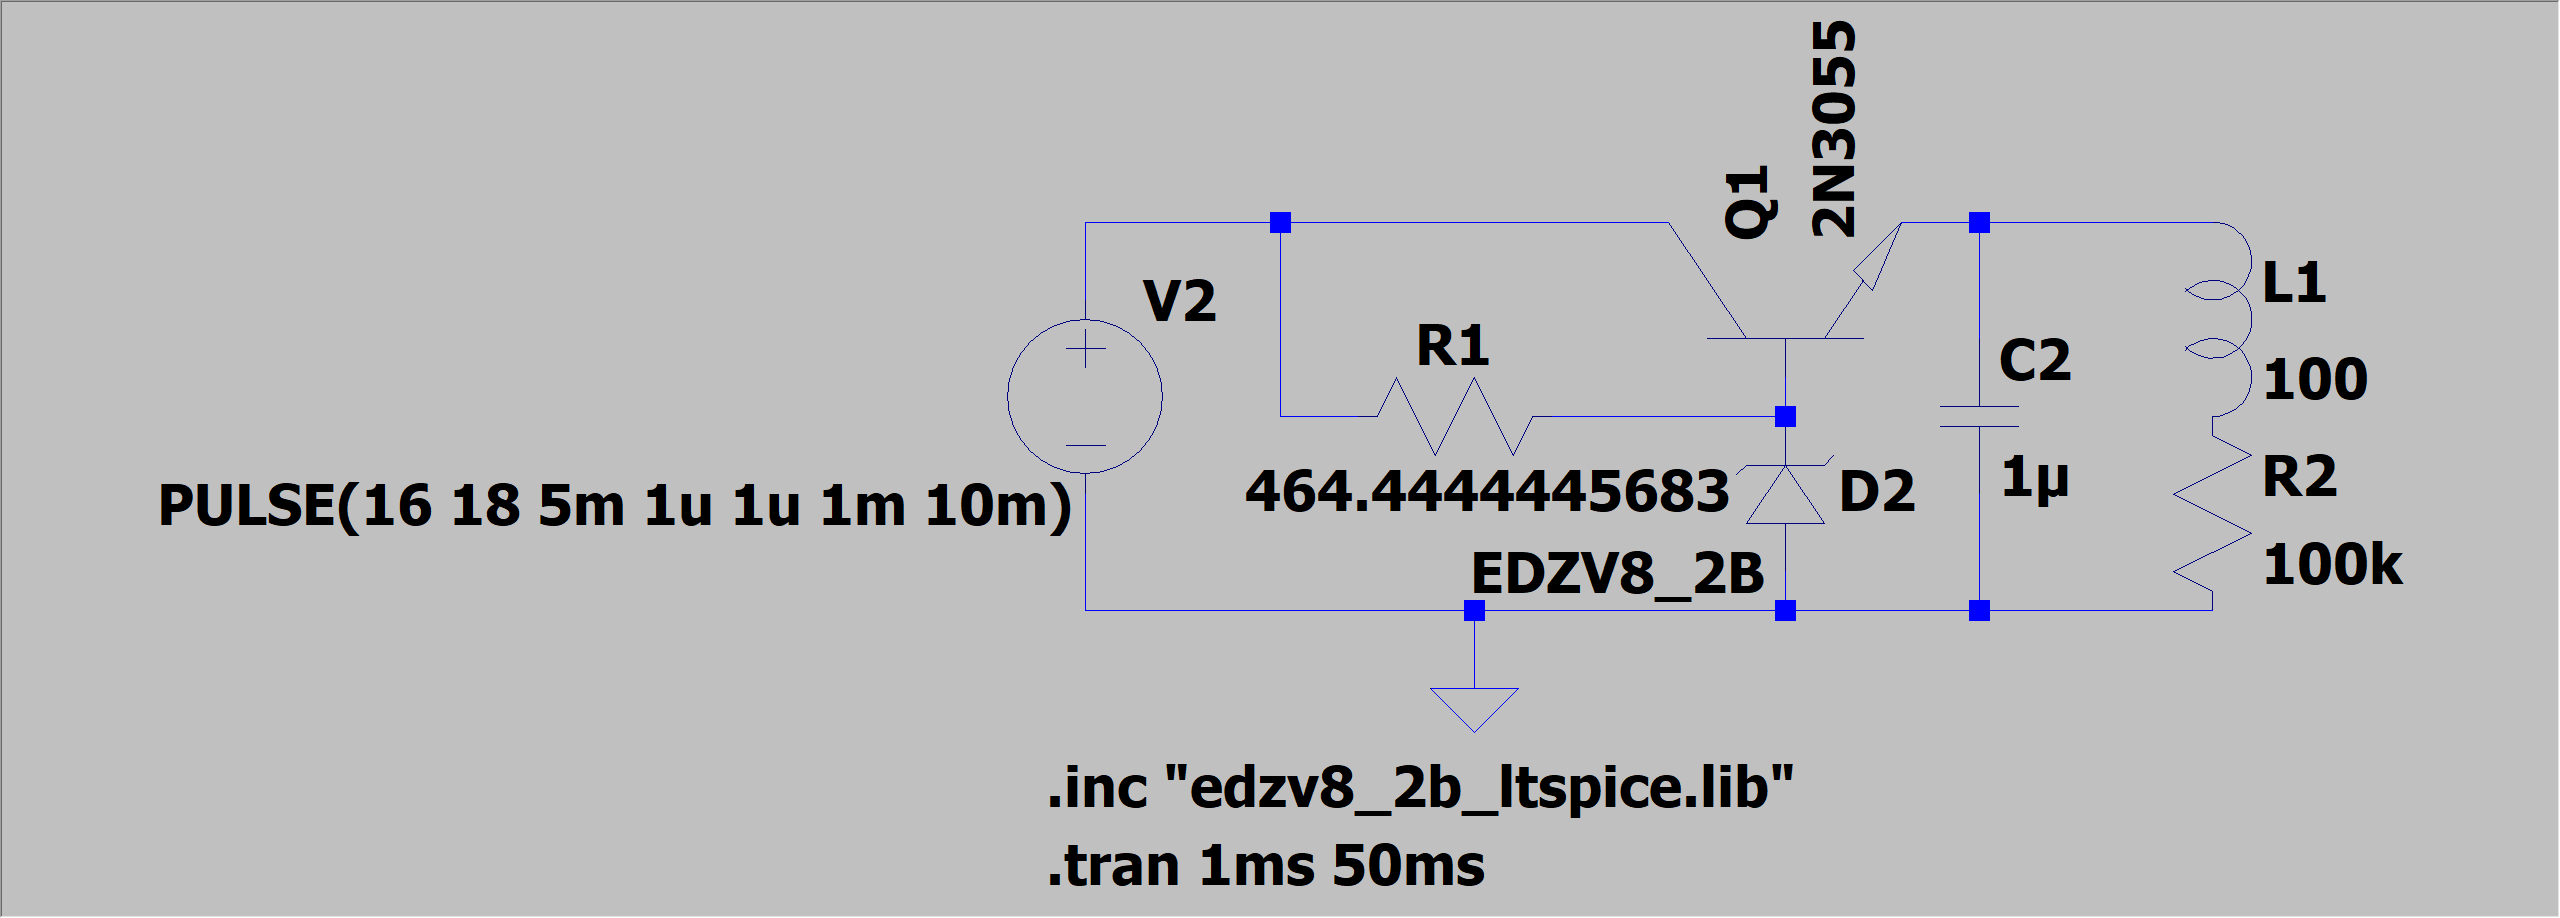
\includegraphics[scale=0.22]{2task_scheme_ALC.png}
        \captionsetup{skip=0pt}
        \caption{Схема параметрического стабилизатора: активно-индуктивно-емкостная нагрузка}
        \label{fig:2task_scheme_ALC}
    \end{figure}
    \noindent Посмотрим выходное напряжение при \textbf{активно-индуктивно-емкостной} нагрузке
    \begin{figure}[H]
        \centering
        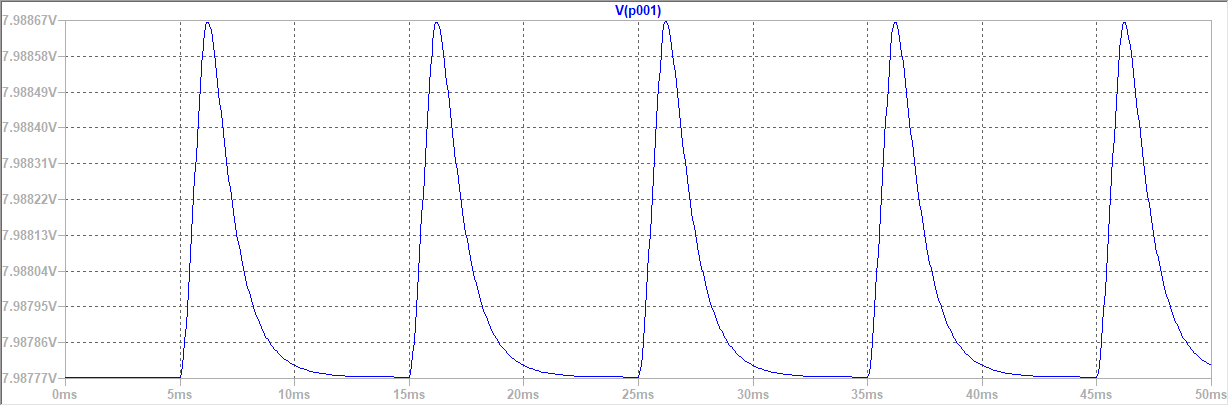
\includegraphics[scale=0.46]{2task_rect_ALC.png}
        \captionsetup{skip=0pt}
        \caption{Выходное напряжение при активно-индуктивно-емкостной скачкообразной нагрузке}
        \label{fig:2task_rect_ALC}
    \end{figure}
    \noindent Результат лучше всего получился на рис. \ref{fig:2task_rect_ALC} и \ref{fig:2task_rect_AC}.
    При увеличении емкости конденсатора пульсации будут сглаживаться еще больше.
\end{document}